% Options for packages loaded elsewhere
\PassOptionsToPackage{unicode}{hyperref}
\PassOptionsToPackage{hyphens}{url}
%
\documentclass[
  ignorenonframetext,
  aspectratio=169,
]{beamer}
\usepackage{pgfpages}
\setbeamertemplate{caption}[numbered]
\setbeamertemplate{caption label separator}{: }
\setbeamercolor{caption name}{fg=normal text.fg}
\beamertemplatenavigationsymbolshorizontal
% Prevent slide breaks in the middle of a paragraph
\widowpenalties 1 10000
\raggedbottom
\setbeamertemplate{part page}{
  \centering
  \begin{beamercolorbox}[sep=16pt,center]{part title}
    \usebeamerfont{part title}\insertpart\par
  \end{beamercolorbox}
}
\setbeamertemplate{section page}{
  \centering
  \begin{beamercolorbox}[sep=12pt,center]{part title}
    \usebeamerfont{section title}\insertsection\par
  \end{beamercolorbox}
}
\setbeamertemplate{subsection page}{
  \centering
  \begin{beamercolorbox}[sep=8pt,center]{part title}
    \usebeamerfont{subsection title}\insertsubsection\par
  \end{beamercolorbox}
}
\AtBeginPart{
  \frame{\partpage}
}
\AtBeginSection{
  \ifbibliography
  \else
    \frame{\sectionpage}
  \fi
}
\AtBeginSubsection{
  \frame{\subsectionpage}
}

\usepackage{amsmath,amssymb}
\usepackage{iftex}
\ifPDFTeX
  \usepackage[T1]{fontenc}
  \usepackage[utf8]{inputenc}
  \usepackage{textcomp} % provide euro and other symbols
\else % if luatex or xetex
  \usepackage{unicode-math}
  \defaultfontfeatures{Scale=MatchLowercase}
  \defaultfontfeatures[\rmfamily]{Ligatures=TeX,Scale=1}
\fi
\usepackage{lmodern}
\ifPDFTeX\else  
    % xetex/luatex font selection
\fi
% Use upquote if available, for straight quotes in verbatim environments
\IfFileExists{upquote.sty}{\usepackage{upquote}}{}
\IfFileExists{microtype.sty}{% use microtype if available
  \usepackage[]{microtype}
  \UseMicrotypeSet[protrusion]{basicmath} % disable protrusion for tt fonts
}{}
\usepackage{xcolor}
\newif\ifbibliography
\setlength{\emergencystretch}{3em} % prevent overfull lines
\setcounter{secnumdepth}{-\maxdimen} % remove section numbering


\providecommand{\tightlist}{%
  \setlength{\itemsep}{0pt}\setlength{\parskip}{0pt}}\usepackage{longtable,booktabs,array}
\usepackage{calc} % for calculating minipage widths
\usepackage{caption}
% Make caption package work with longtable
\makeatletter
\def\fnum@table{\tablename~\thetable}
\makeatother
\usepackage{graphicx}
\makeatletter
\def\maxwidth{\ifdim\Gin@nat@width>\linewidth\linewidth\else\Gin@nat@width\fi}
\def\maxheight{\ifdim\Gin@nat@height>\textheight\textheight\else\Gin@nat@height\fi}
\makeatother
% Scale images if necessary, so that they will not overflow the page
% margins by default, and it is still possible to overwrite the defaults
% using explicit options in \includegraphics[width, height, ...]{}
\setkeys{Gin}{width=\maxwidth,height=\maxheight,keepaspectratio}
% Set default figure placement to htbp
\makeatletter
\def\fps@figure{htbp}
\makeatother

\IfFileExists{plex-otf.sty}{
  %% Full TeXlive
  % \usepackage[%
  %   % math,
  %   RM={Scale=0.94},SS={Scale=0.94},SScon={Scale=0.94},TT={Scale=MatchLowercase,FakeStretch=0.9},DefaultFeatures={Ligatures=Common}
  % ]{plex-otf}
}{
  %% TinyTeX
  \usepackage{libertine}
}

%%% Load theme
% https://deic.uab.cat/~iblanes/beamer_gallery/
\IfFileExists{beamerthemegotham.sty}{
  %% Full TeXlive
  \usetheme{gotham}
  \gothamset{
    numbering=totalpagenumber,
    parttocframe default=off,
    sectiontocframe default=off,
    subsectiontocframe default=off,
  }
}{
  %% TinyTeX
  \usetheme{Madrid}
}
\usepackage{polyglossia}
\setdefaultlanguage{russian}
\setotherlanguage{english}
\usepackage{fontspec}
\setmainfont{Times New Roman}
\setsansfont{Arial}
\setmonofont{Courier New}
\makeatletter
\@ifpackageloaded{caption}{}{\usepackage{caption}}
\AtBeginDocument{%
\ifdefined\contentsname
  \renewcommand*\contentsname{Содержание}
\else
  \newcommand\contentsname{Содержание}
\fi
\ifdefined\listfigurename
  \renewcommand*\listfigurename{Список иллюстраций}
\else
  \newcommand\listfigurename{Список иллюстраций}
\fi
\ifdefined\listtablename
  \renewcommand*\listtablename{Список таблиц}
\else
  \newcommand\listtablename{Список таблиц}
\fi
\ifdefined\figurename
  \renewcommand*\figurename{Рисунок}
\else
  \newcommand\figurename{Рисунок}
\fi
\ifdefined\tablename
  \renewcommand*\tablename{Таблица}
\else
  \newcommand\tablename{Таблица}
\fi
}
\@ifpackageloaded{float}{}{\usepackage{float}}
\floatstyle{ruled}
\@ifundefined{c@chapter}{\newfloat{codelisting}{h}{lop}}{\newfloat{codelisting}{h}{lop}[chapter]}
\floatname{codelisting}{Список}
\newcommand*\listoflistings{\listof{codelisting}{Листинги}}
\makeatother
\makeatletter
\makeatother
\makeatletter
\@ifpackageloaded{caption}{}{\usepackage{caption}}
\@ifpackageloaded{subcaption}{}{\usepackage{subcaption}}
\makeatother
\ifLuaTeX
\usepackage[bidi=basic]{babel}
\else
\usepackage[bidi=default]{babel}
\fi
\babelprovide[main,import]{russian}
\babelprovide[import]{english}
% get rid of language-specific shorthands (see #6817):
\let\LanguageShortHands\languageshorthands
\def\languageshorthands#1{}
\ifLuaTeX
  \usepackage{selnolig}  % disable illegal ligatures
\fi
\usepackage{csquotes}
\usepackage{bookmark}

\IfFileExists{xurl.sty}{\usepackage{xurl}}{} % add URL line breaks if available
\urlstyle{same} % disable monospaced font for URLs
\hypersetup{
  pdftitle={Презентация по лабораторной работе1},
  pdfauthor={Нджову Нелиа},
  pdflang={ru},
  hidelinks,
  pdfcreator={LaTeX via pandoc}}

\title{Презентация по лабораторной работе1}
\subtitle{Математическое моделирование}
\author{Нджову Нелиа}
\date{}

\begin{document}
\frame{\titlepage}

\renewcommand*\contentsname{Содержание}
\begin{frame}[allowframebreaks]
  \frametitle{Содержание}
  \tableofcontents[hideallsubsections]
\end{frame}
\begin{frame}{Цель работы}
\phantomsection\label{ux446ux435ux43bux44c-ux440ux430ux431ux43eux442ux44b}
Изучить модель экспоненциального роста, провести параметрическое
исследование влияния коэффициента роста αα на динамику системы, а также
освоить современные практики воспроизводимых исследований (литературное
программирование, DrWatson, Git) при выполнении лабораторных работ.
\end{frame}

\begin{frame}{Задание}
\phantomsection\label{ux437ux430ux434ux430ux43dux438ux435}
\begin{enumerate}[<+->]
\item
  Настройка git
\item
  Рабочее пространство лабораторной работы
\item
  Создание проекта DrWatson для лабораторных
\item
  Модель экспоненциального роста
\end{enumerate}
\end{frame}

\begin{frame}{1. Настройка git}
\phantomsection\label{ux43dux430ux441ux442ux440ux43eux439ux43aux430-git}
Из моих предыдущих лабораторных работ я уже установил git и gh и
выполнил базовую настройку. Итак, для этой лабораторной работы я начал с
создания учетной записи на gitverse и заполнения необходимой
информации(рис.1).

\begin{figure}

\centering{

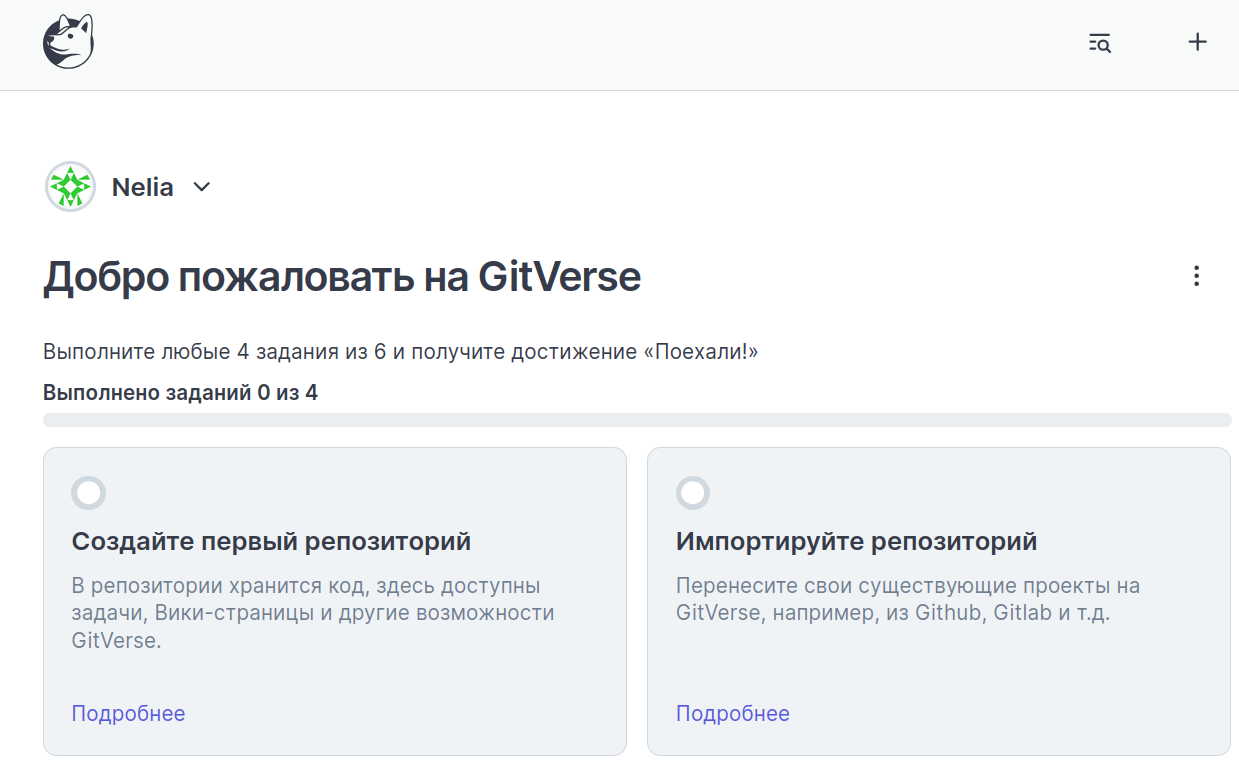
\includegraphics[width=0.7\textwidth,height=\textheight]{image/fig-002.png}

}

\caption{\label{fig-001}Создание учетной записи на gitverse}

\end{figure}%
\end{frame}

\begin{frame}{1. Настройка git}
\phantomsection\label{ux43dux430ux441ux442ux440ux43eux439ux43aux430-git-1}
Я авторизуюсь с помощью команды gh auth login. Утилита задала мне
несколько вопросов, и в итоге я авторизовался через браузер(рис.2)

\begin{figure}

\centering{

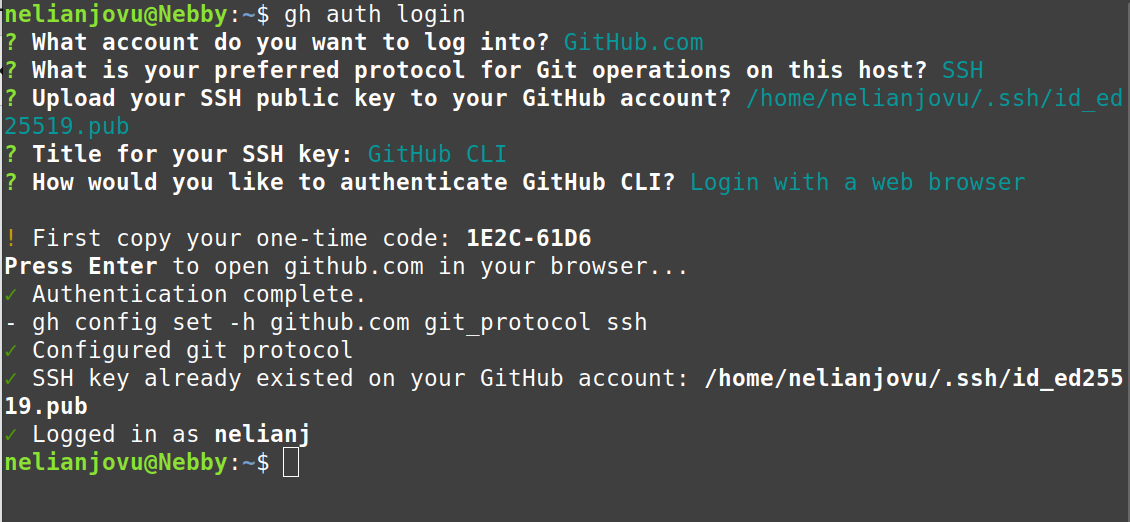
\includegraphics[width=0.7\textwidth,height=\textheight]{image/fig-005.png}

}

\caption{\label{fig-002}Авторизация учетной записи}

\end{figure}%
\end{frame}

\begin{frame}{1. Настройка git}
\phantomsection\label{ux43dux430ux441ux442ux440ux43eux439ux43aux430-git-2}
Я создаю ключ ssh для доступа к github(рис.3)

\begin{figure}

\centering{


\includegraphics[width=0.7\textwidth,height=\textheight]{image/fig-007.png}

}

\caption{\label{fig-003}Ключ для доступа к github}

\end{figure}%
\end{frame}

\begin{frame}{1. Настройка git}
\phantomsection\label{ux43dux430ux441ux442ux440ux43eux439ux43aux430-git-3}
Я добавляю ключ ssh в агента(рис. 4)

\begin{figure}

\centering{


\includegraphics[width=0.7\textwidth,height=\textheight]{image/fig-008.png}

}

\caption{\label{fig-004}Добавление ключа в агента}

\end{figure}%
\end{frame}

\begin{frame}{1. Настройка git}
\phantomsection\label{ux43dux430ux441ux442ux440ux43eux439ux43aux430-git-4}
Я добавляю ключ ssh к вашей учетной записи на gitverse через
веб-интерфейс. Затем используйте команду, чтобы добавить ключ ssh к
вашей учетной записи на github(рис. 5 и 6)

\begin{figure}

\centering{

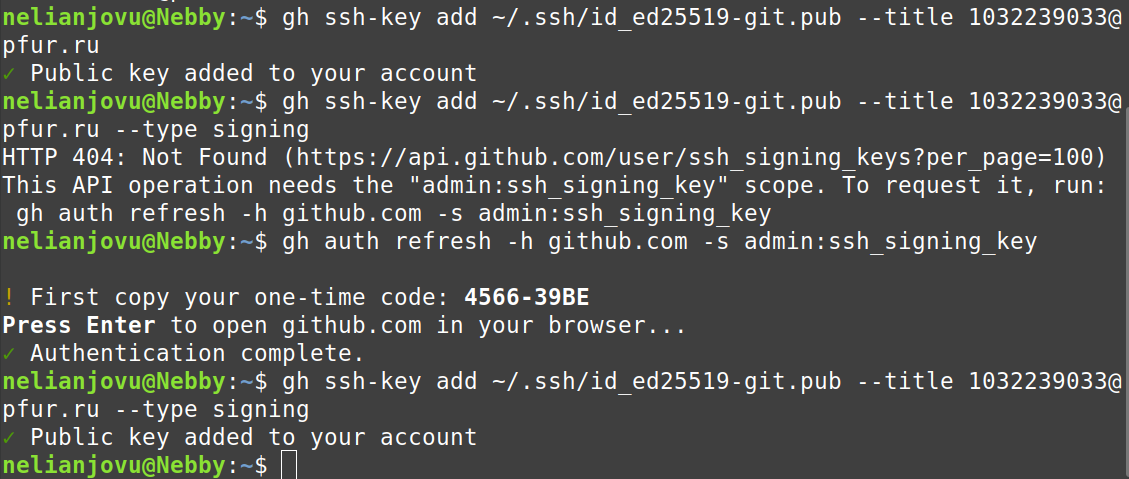
\includegraphics[width=0.7\textwidth,height=\textheight]{image/fig-011.png}

}

\caption{\label{fig-005}Добавление ключа на gitverse}

\end{figure}%
\end{frame}

\begin{frame}{1. Настройка git}
\phantomsection\label{ux43dux430ux441ux442ux440ux43eux439ux43aux430-git-5}
\begin{figure}

\centering{

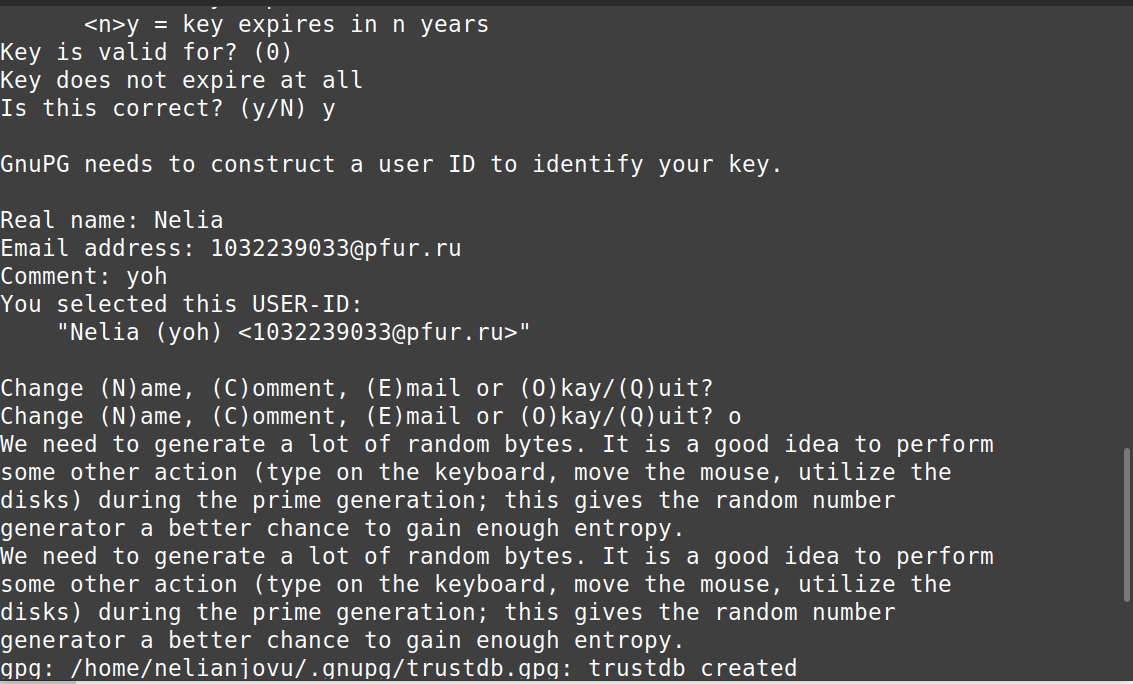
\includegraphics[width=0.7\textwidth,height=\textheight]{image/fig-013.png}

}

\caption{\label{fig-006}Добавление ключа на github}

\end{figure}%
\end{frame}

\begin{frame}{1. Настройка git}
\phantomsection\label{ux43dux430ux441ux442ux440ux43eux439ux43aux430-git-6}
Я генерирую ключ gpg, выбирая параметры, указанные в руководстве по
лабораторной работе(рис. 7)

\begin{figure}

\centering{

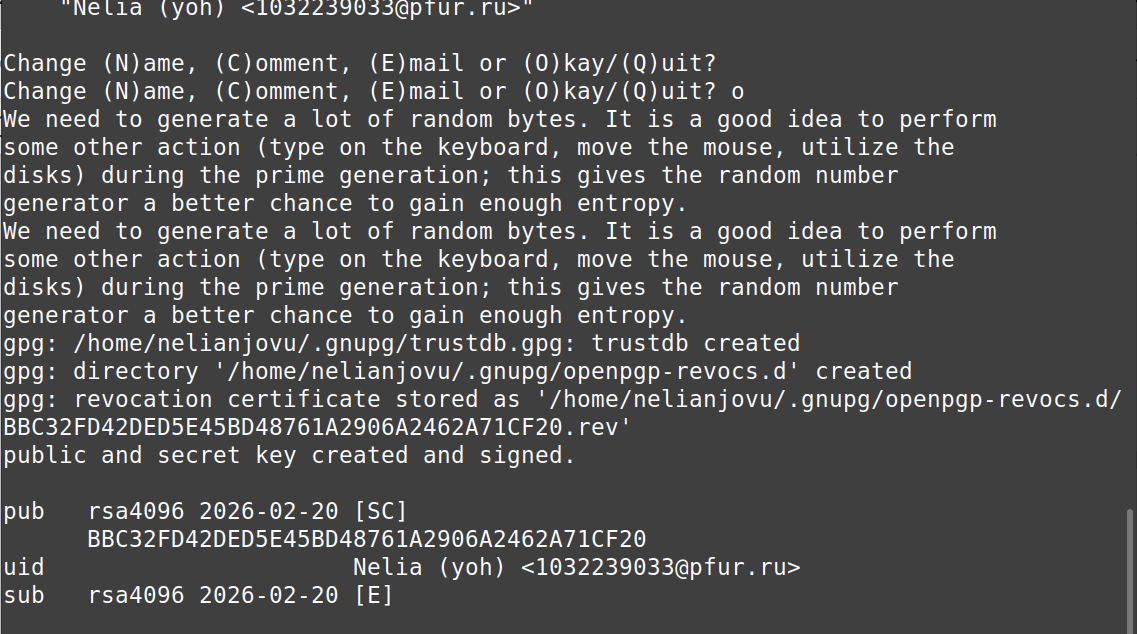
\includegraphics[width=0.7\textwidth,height=\textheight]{image/fig-014.png}

}

\caption{\label{fig-007}генерация ключа gpg}

\end{figure}%
\end{frame}

\begin{frame}{1. Настройка git}
\phantomsection\label{ux43dux430ux441ux442ux440ux43eux439ux43aux430-git-7}
Я вывожу список ключей и копирую отпечаток пальца (который находится под
строкой, начинающейся с sec) закрытого ключа.(рис. 8)

\begin{figure}

\centering{

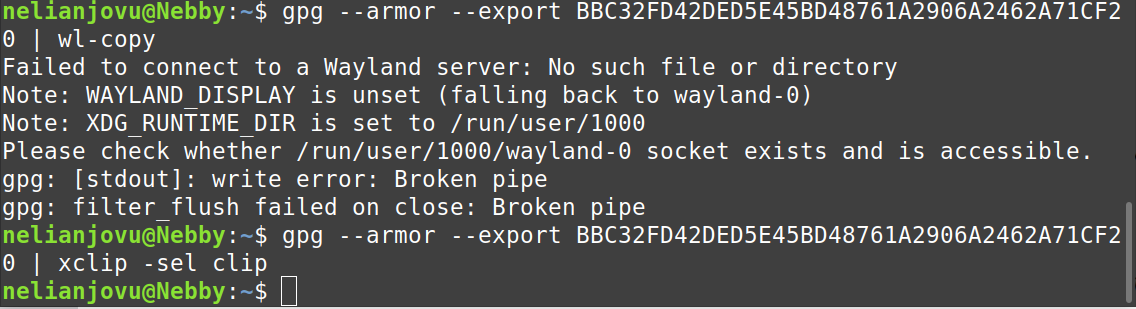
\includegraphics[width=0.7\textwidth,height=\textheight]{image/fig-017.png}

}

\caption{\label{fig-008}список ключей}

\end{figure}%
\end{frame}

\begin{frame}{1. Настройка git}
\phantomsection\label{ux43dux430ux441ux442ux440ux43eux439ux43aux430-git-8}
Я копирую сгенерированный PGP-ключ в буфер обмена. Я использую xclip,
потому что wl-copy выдал ошибку(рис. 9)

\begin{figure}

\centering{

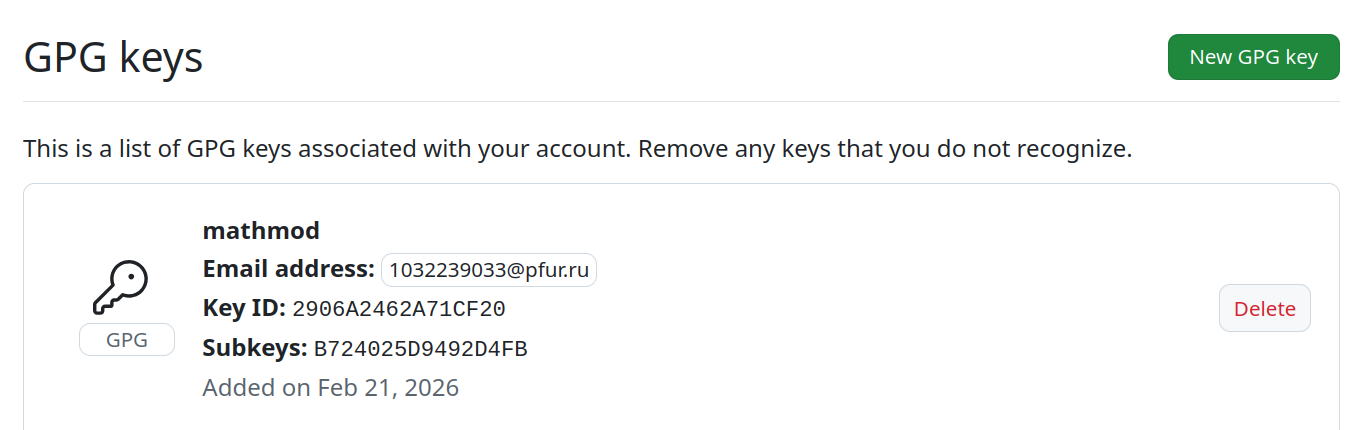
\includegraphics[width=0.7\textwidth,height=\textheight]{image/fig-019.png}

}

\caption{\label{fig-009}копирование ключа}

\end{figure}%
\end{frame}

\begin{frame}{1. Настройка git}
\phantomsection\label{ux43dux430ux441ux442ux440ux43eux439ux43aux430-git-9}
Я добавляю сгенерированный ключ gpg в github и gitverse(рис. 10 и 11)

\begin{figure}

\centering{

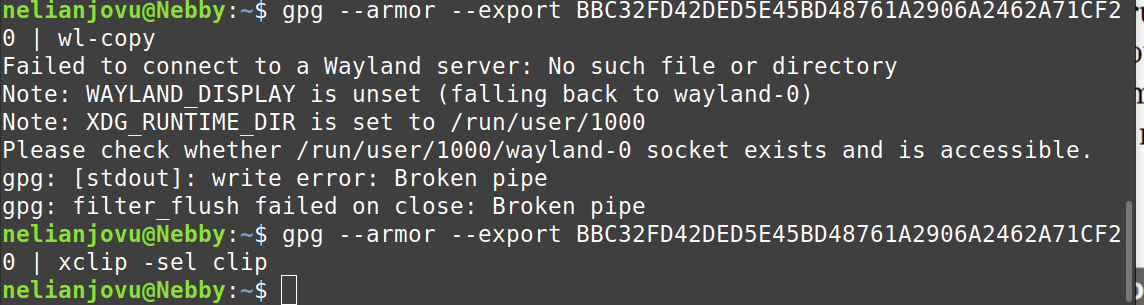
\includegraphics[width=0.7\textwidth,height=\textheight]{image/fig-020.png}

}

\caption{\label{fig-010}Добавление ключа на gitverse}

\end{figure}%
\end{frame}

\begin{frame}{1. Настройка git}
\phantomsection\label{ux43dux430ux441ux442ux440ux43eux439ux43aux430-git-10}
\begin{figure}

\centering{

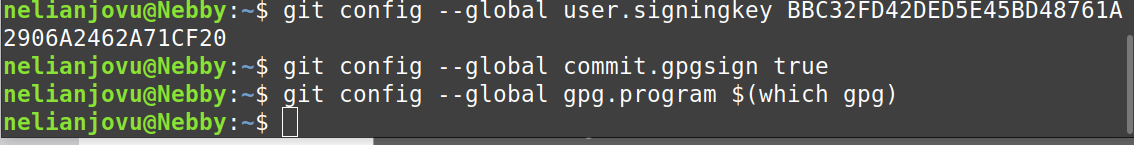
\includegraphics[width=0.7\textwidth,height=\textheight]{image/fig-021.png}

}

\caption{\label{fig-011}Добавление ключа на github}

\end{figure}%
\end{frame}

\begin{frame}{1. Настройка git}
\phantomsection\label{ux43dux430ux441ux442ux440ux43eux439ux43aux430-git-11}
Используя электронное письмо, подключенное к моей учетной записи, я
говорю Git использовать его при подписании коммитов(рис. 12)

\begin{figure}

\centering{

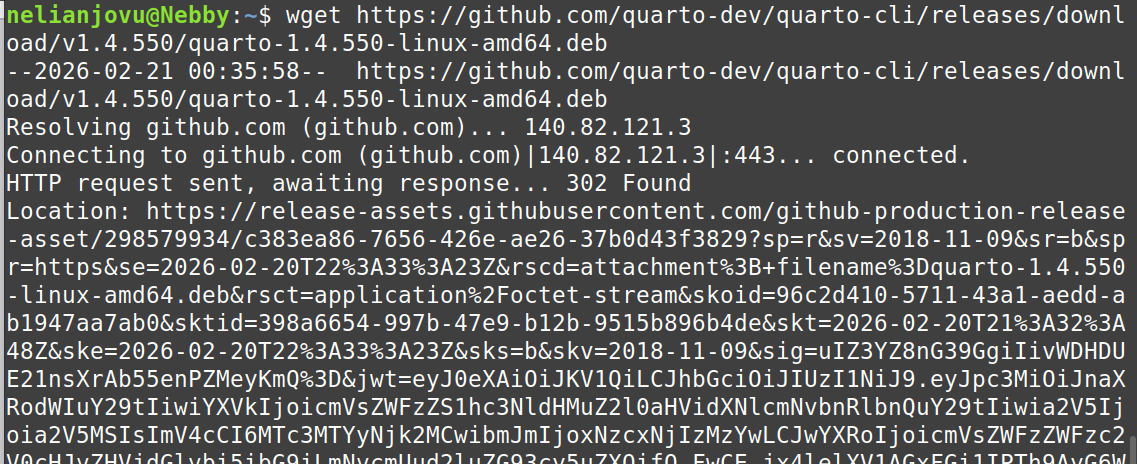
\includegraphics[width=0.7\textwidth,height=\textheight]{image/fig-023.png}

}

\caption{\label{fig-012}автоматические подписи git-коммитов}

\end{figure}%
\end{frame}

\begin{frame}{2. Рабочее пространство лабораторной работы}
\phantomsection\label{ux440ux430ux431ux43eux447ux435ux435-ux43fux440ux43eux441ux442ux440ux430ux43dux441ux442ux432ux43e-ux43bux430ux431ux43eux440ux430ux442ux43eux440ux43dux43eux439-ux440ux430ux431ux43eux442ux44b}
Я устанавливаю пакет, который поставляется с инструментами разработки
для linux mint(рис. 13)

\begin{figure}

\centering{

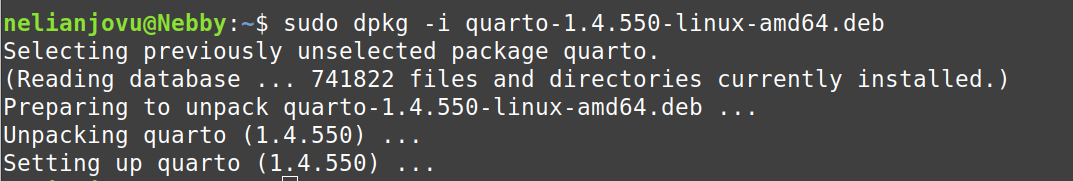
\includegraphics[width=0.7\textwidth,height=\textheight]{image/fig-024.png}

}

\caption{\label{fig-013}уствновка инструменты разработки}

\end{figure}%
\end{frame}

\begin{frame}{2. Рабочее пространство лабораторной работы}
\phantomsection\label{ux440ux430ux431ux43eux447ux435ux435-ux43fux440ux43eux441ux442ux440ux430ux43dux441ux442ux432ux43e-ux43bux430ux431ux43eux440ux430ux442ux43eux440ux43dux43eux439-ux440ux430ux431ux43eux442ux44b-1}
Затем я устанавливаю quarto. Quarto - это инструмент для научной
публикации с открытым исходным кодом, который позволяет создавать
профессиональные отчеты, объединяя текст, код и результаты в одном
документе, с поддержкой Julia, Python и R(рис. 14)

\begin{figure}

\centering{

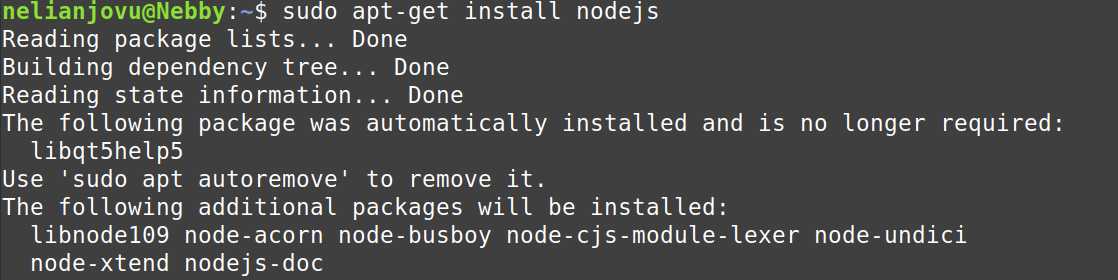
\includegraphics[width=0.7\textwidth,height=\textheight]{image/fig-025.png}

}

\caption{\label{fig-014}уствновка quarto}

\end{figure}%
\end{frame}

\begin{frame}{2. Рабочее пространство лабораторной работы}
\phantomsection\label{ux440ux430ux431ux43eux447ux435ux435-ux43fux440ux43eux441ux442ux440ux430ux43dux441ux442ux432ux43e-ux43bux430ux431ux43eux440ux430ux442ux43eux440ux43dux43eux439-ux440ux430ux431ux43eux442ux44b-2}
Наконец, я устанавливаю nodejs, yarn и pnpm(рис. 15, 16 и 17)

\begin{figure}

\centering{

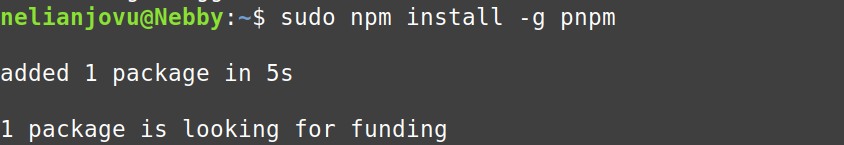
\includegraphics[width=0.7\textwidth,height=\textheight]{image/fig-027.png}

}

\caption{\label{fig-015}уствновка nodejs}

\end{figure}%
\end{frame}

\begin{frame}{2. Рабочее пространство лабораторной работы}
\phantomsection\label{ux440ux430ux431ux43eux447ux435ux435-ux43fux440ux43eux441ux442ux440ux430ux43dux441ux442ux432ux43e-ux43bux430ux431ux43eux440ux430ux442ux43eux440ux43dux43eux439-ux440ux430ux431ux43eux442ux44b-3}
\begin{figure}

\centering{

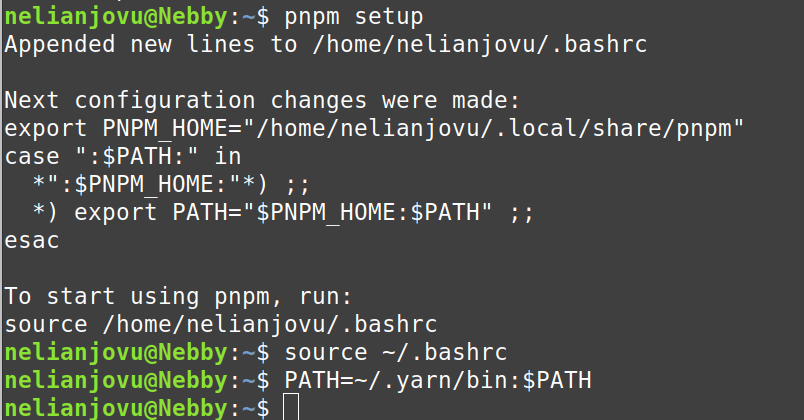
\includegraphics[width=0.7\textwidth,height=\textheight]{image/fig-028.png}

}

\caption{\label{fig-016}уствновка yarn}

\end{figure}%
\end{frame}

\begin{frame}{2. Рабочее пространство лабораторной работы}
\phantomsection\label{ux440ux430ux431ux43eux447ux435ux435-ux43fux440ux43eux441ux442ux440ux430ux43dux441ux442ux432ux43e-ux43bux430ux431ux43eux440ux430ux442ux43eux440ux43dux43eux439-ux440ux430ux431ux43eux442ux44b-4}
\begin{figure}

\centering{

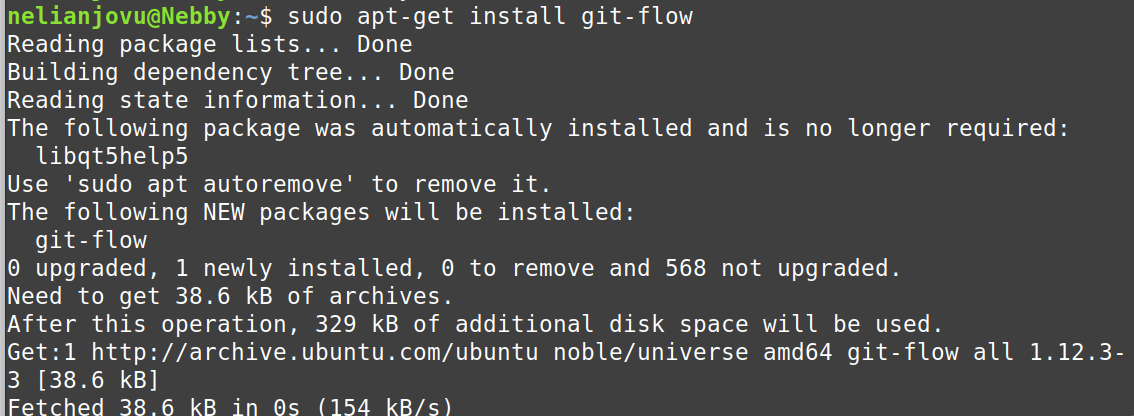
\includegraphics[width=0.7\textwidth,height=\textheight]{image/fig-029.png}

}

\caption{\label{fig-017}уствновка pnpm}

\end{figure}%
\end{frame}

\begin{frame}{2. Рабочее пространство лабораторной работы}
\phantomsection\label{ux440ux430ux431ux43eux447ux435ux435-ux43fux440ux43eux441ux442ux440ux430ux43dux441ux442ux432ux43e-ux43bux430ux431ux43eux440ux430ux442ux43eux440ux43dux43eux439-ux440ux430ux431ux43eux442ux44b-5}
Для работы с Node.js Я добавляю каталог с исполняемыми файлами,
установленными менеджером пакетов, в переменную PATH(рис. 18)

\begin{figure}

\centering{

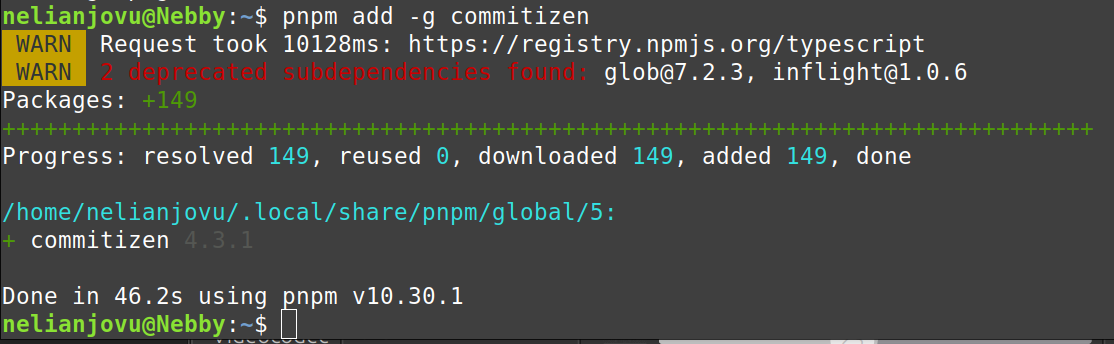
\includegraphics[width=0.7\textwidth,height=\textheight]{image/fig-030.png}

}

\caption{\label{fig-018}настройка nodejs}

\end{figure}%
\end{frame}

\begin{frame}{2. Рабочее пространство лабораторной работы}
\phantomsection\label{ux440ux430ux431ux43eux447ux435ux435-ux43fux440ux43eux441ux442ux440ux430ux43dux441ux442ux432ux43e-ux43bux430ux431ux43eux440ux430ux442ux43eux440ux43dux43eux439-ux440ux430ux431ux43eux442ux44b-6}
Я устанавливаю gitflow. Gitflow - это модель ветвления для Git, которая
обеспечивает структурированный рабочий процесс с использованием
выделенных ветвей для функций, релизов и исправлений, помогая командам
управлять параллельной разработкой и поддерживать стабильный код(рис.
19)

\begin{figure}

\centering{

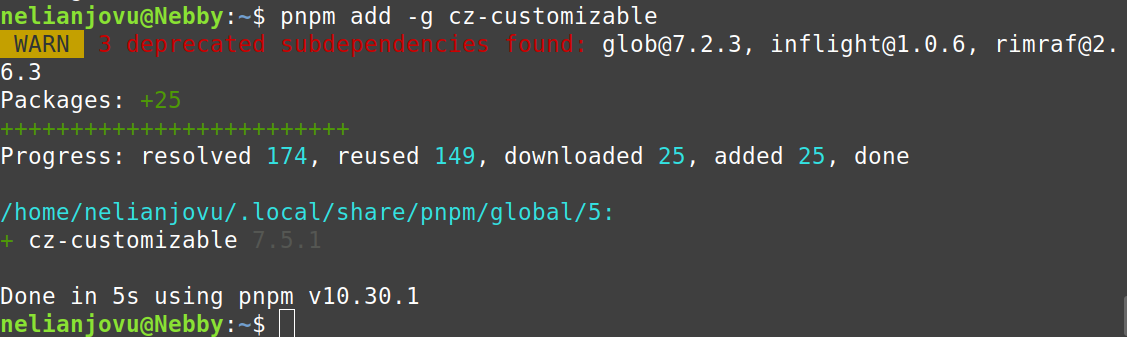
\includegraphics[width=0.7\textwidth,height=\textheight]{image/fig-031.png}

}

\caption{\label{fig-019}уствновка gitflow}

\end{figure}%
\end{frame}

\begin{frame}{2. Рабочее пространство лабораторной работы}
\phantomsection\label{ux440ux430ux431ux43eux447ux435ux435-ux43fux440ux43eux441ux442ux440ux430ux43dux441ux442ux432ux43e-ux43bux430ux431ux43eux440ux430ux442ux43eux440ux43dux43eux439-ux440ux430ux431ux43eux442ux44b-7}
Следуя инструкциям руководства, я использую команды, которые помогают
форматировать коммиты, одновременно с этим устанавливается git-cz,
который мы будем использовать для коммитов(рис. 20)

\begin{figure}

\centering{

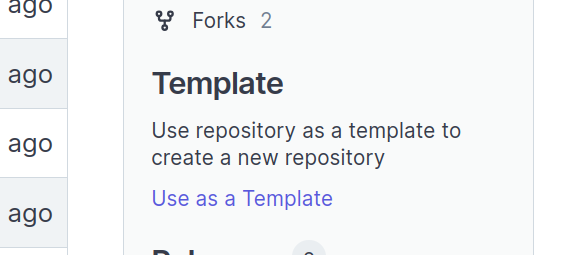
\includegraphics[width=0.7\textwidth,height=\textheight]{image/fig-033.png}

}

\caption{\label{fig-020}форматировка коммиты}

\end{figure}%
\end{frame}

\begin{frame}{2. Рабочее пространство лабораторной работы}
\phantomsection\label{ux440ux430ux431ux43eux447ux435ux435-ux43fux440ux43eux441ux442ux440ux430ux43dux441ux442ux432ux43e-ux43bux430ux431ux43eux440ux430ux442ux43eux440ux43dux43eux439-ux440ux430ux431ux43eux442ux44b-8}
Команда на скриншоте позволяет мне более глубоко настроить
форматирование коммитов(рис. 21)

\begin{figure}

\centering{

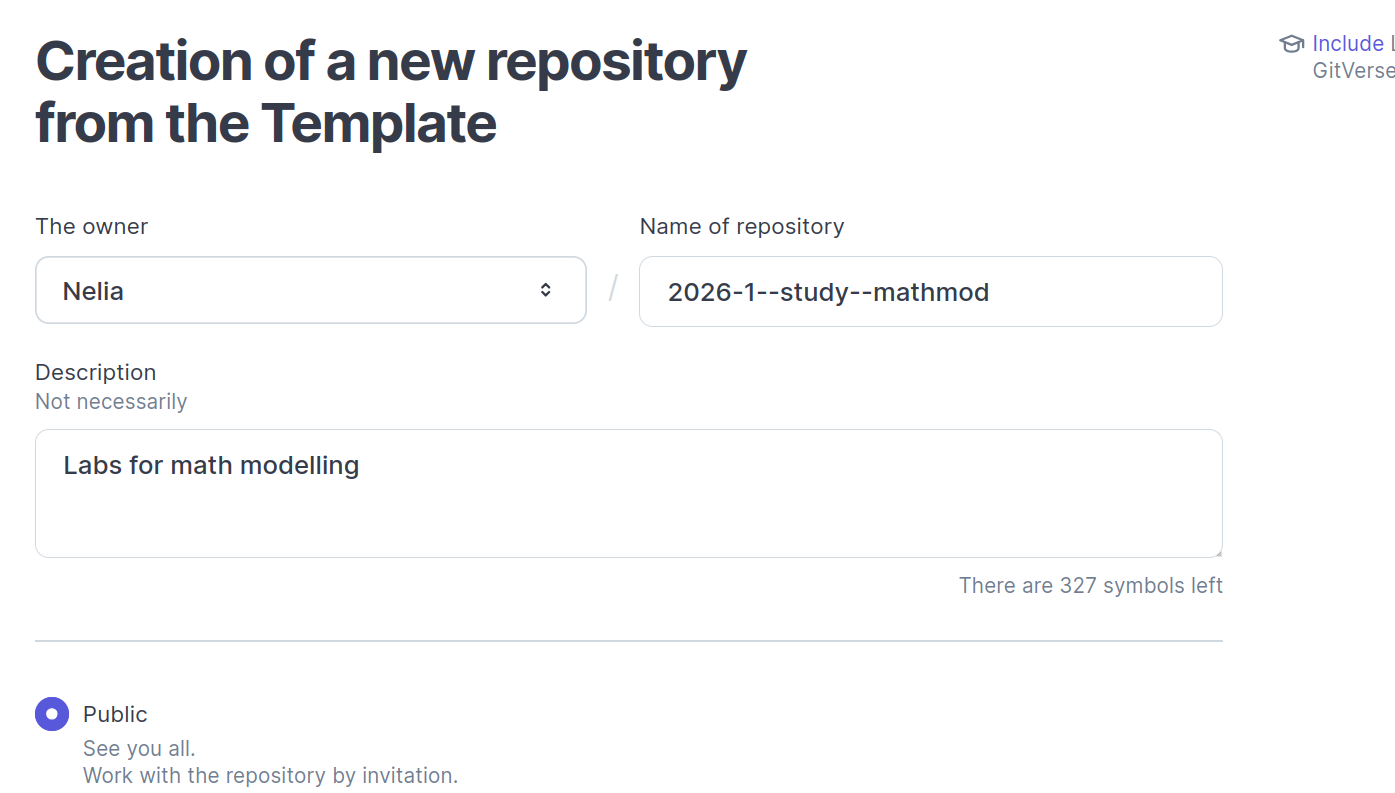
\includegraphics[width=0.7\textwidth,height=\textheight]{image/fig-034.png}

}

\caption{\label{fig-021}форматировка коммиты}

\end{figure}%
\end{frame}

\begin{frame}{2. Рабочее пространство лабораторной работы}
\phantomsection\label{ux440ux430ux431ux43eux447ux435ux435-ux43fux440ux43eux441ux442ux440ux430ux43dux441ux442ux432ux43e-ux43bux430ux431ux43eux440ux430ux442ux43eux440ux43dux43eux439-ux440ux430ux431ux43eux442ux44b-9}
Эта команда автоматизирует изменение номера версии(рис. 22)

\begin{figure}

\centering{

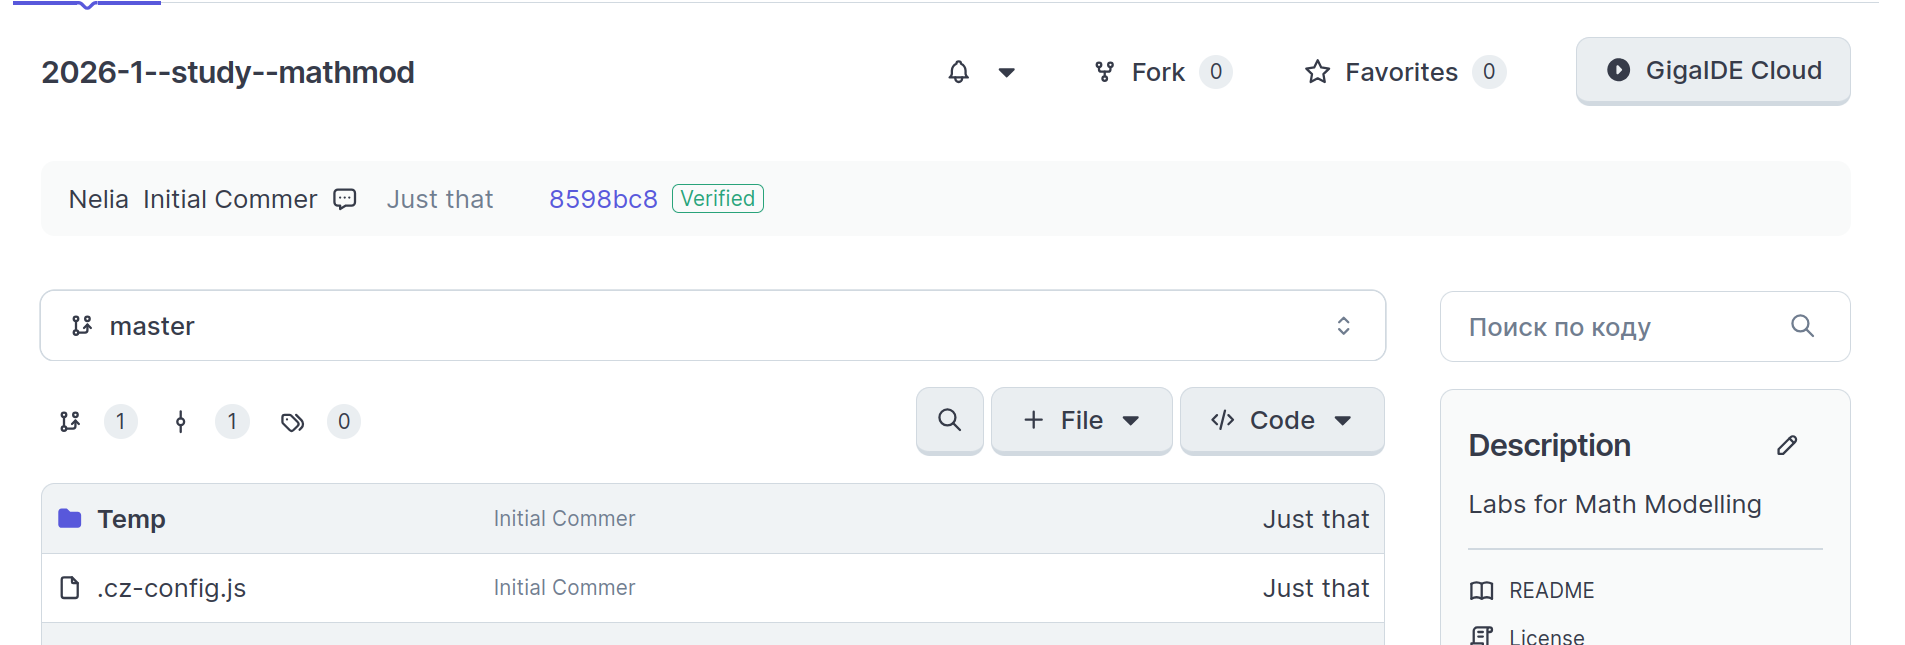
\includegraphics[width=0.7\textwidth,height=\textheight]{image/fig-035.png}

}

\caption{\label{fig-022}форматировка коммиты}

\end{figure}%
\end{frame}

\begin{frame}{2. Рабочее пространство лабораторной работы}
\phantomsection\label{ux440ux430ux431ux43eux447ux435ux435-ux43fux440ux43eux441ux442ux440ux430ux43dux441ux442ux432ux43e-ux43bux430ux431ux43eux440ux430ux442ux43eux440ux43dux43eux439-ux440ux430ux431ux43eux442ux44b-10}
Я использую шаблон, указанный в руководстве, для создания нового
репозитория на gitverse(рис. 23)

\begin{figure}

\centering{

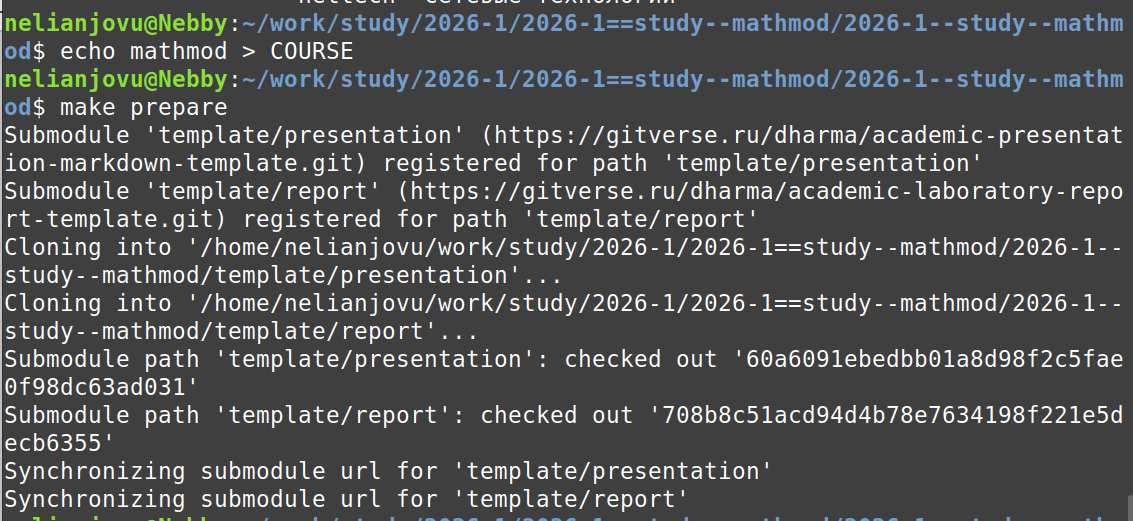
\includegraphics[width=0.7\textwidth,height=\textheight]{image/fig-038.png}

}

\caption{\label{fig-023}создание нового репозитория}

\end{figure}%
\end{frame}

\begin{frame}{2. Рабочее пространство лабораторной работы}
\phantomsection\label{ux440ux430ux431ux43eux447ux435ux435-ux43fux440ux43eux441ux442ux440ux430ux43dux441ux442ux432ux43e-ux43bux430ux431ux43eux440ux430ux442ux43eux440ux43dux43eux439-ux440ux430ux431ux43eux442ux44b-11}
Я создаю файл для своей лабораторной работы, а затем клонирую
репозиторий(рис. 24)

\begin{figure}

\centering{

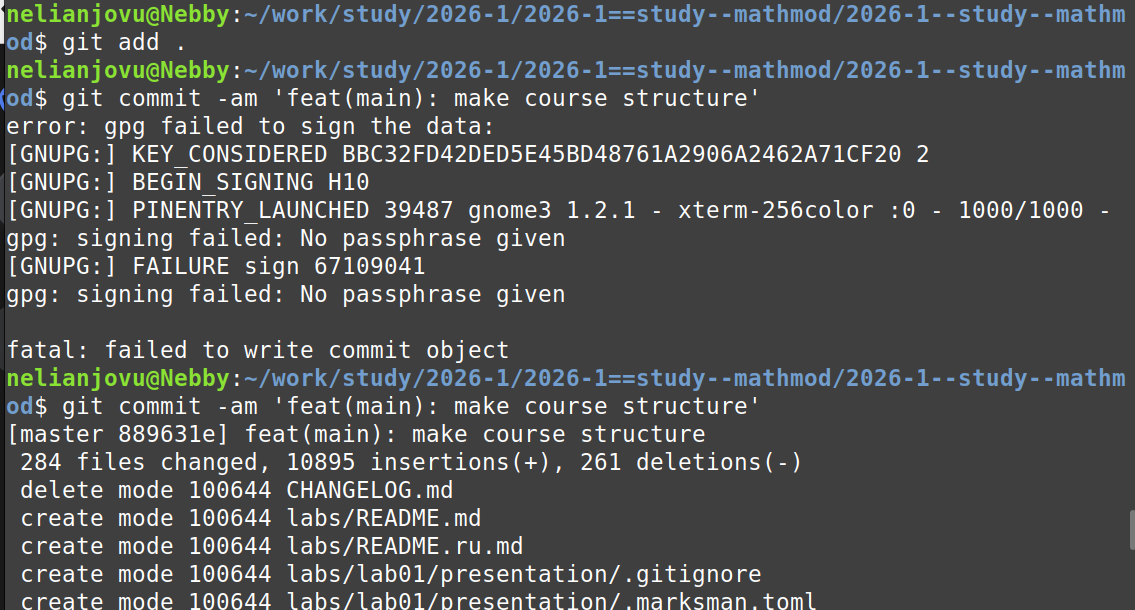
\includegraphics[width=0.7\textwidth,height=\textheight]{image/fig-039.png}

}

\caption{\label{fig-024}клонирование репозитория}

\end{figure}%
\end{frame}

\begin{frame}{2. Рабочее пространство лабораторной работы}
\phantomsection\label{ux440ux430ux431ux43eux447ux435ux435-ux43fux440ux43eux441ux442ux440ux430ux43dux441ux442ux432ux43e-ux43bux430ux431ux43eux440ux430ux442ux43eux440ux43dux43eux439-ux440ux430ux431ux43eux442ux44b-12}
Я просматриваю доступные цели создания и список доступных курсов(рис.
25)

\begin{figure}

\centering{

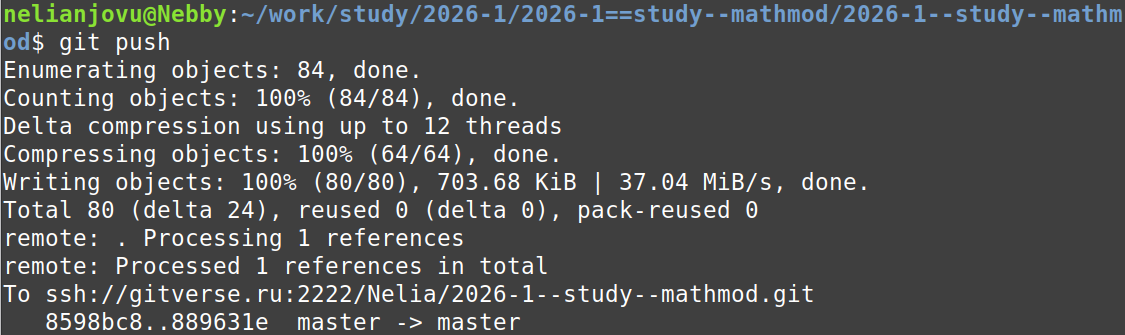
\includegraphics[width=0.7\textwidth,height=\textheight]{image/fig-040.png}

}

\caption{\label{fig-025}проверка доступных целей и списка курсов}

\end{figure}%
\end{frame}

\begin{frame}{2. Рабочее пространство лабораторной работы}
\phantomsection\label{ux440ux430ux431ux43eux447ux435ux435-ux43fux440ux43eux441ux442ux440ux430ux43dux441ux442ux432ux43e-ux43bux430ux431ux43eux440ux430ux442ux43eux440ux43dux43eux439-ux440ux430ux431ux43eux442ux44b-13}
Я захожу в свой каталог лабораторных работ и инициализирую курс(рис. 26)

\begin{figure}

\centering{

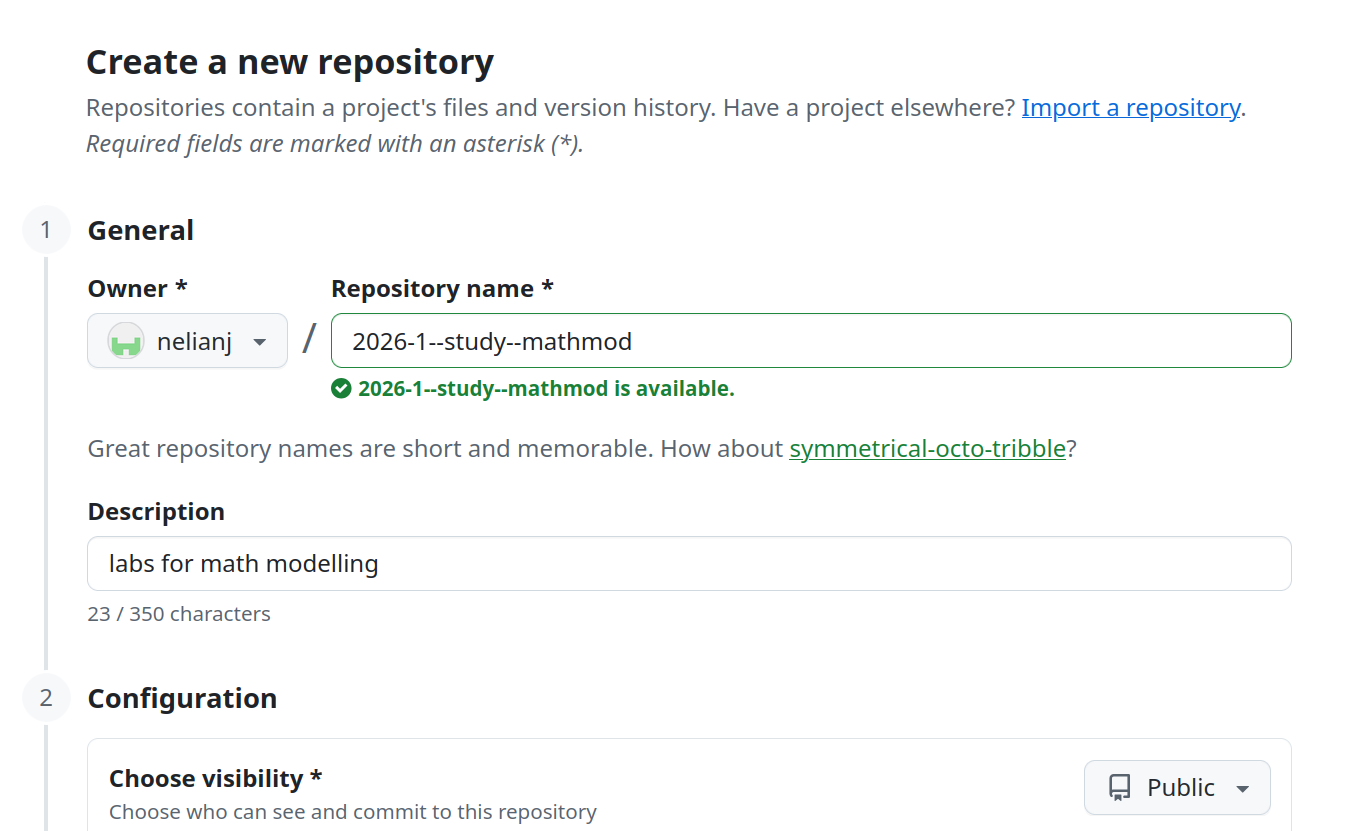
\includegraphics[width=0.7\textwidth,height=\textheight]{image/fig-041.png}

}

\caption{\label{fig-026}инициализация курса}

\end{figure}%
\end{frame}

\begin{frame}{2. Рабочее пространство лабораторной работы}
\phantomsection\label{ux440ux430ux431ux43eux447ux435ux435-ux43fux440ux43eux441ux442ux440ux430ux43dux441ux442ux432ux43e-ux43bux430ux431ux43eux440ux430ux442ux43eux440ux43dux43eux439-ux440ux430ux431ux43eux442ux44b-14}
Я отправляю файлы на сервер(рис. 27)

\begin{figure}

\centering{

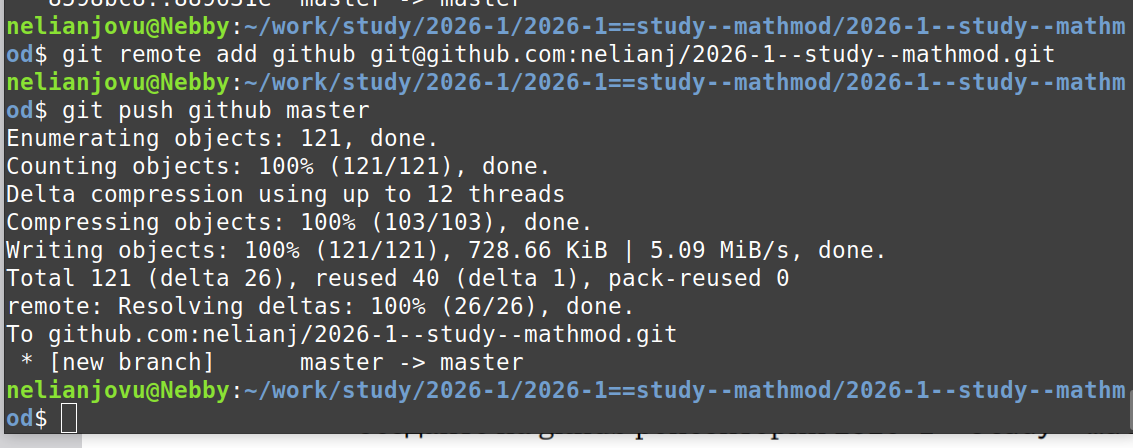
\includegraphics[width=0.7\textwidth,height=\textheight]{image/fig-042.png}

}

\caption{\label{fig-027}отправка файлов}

\end{figure}%
\end{frame}

\begin{frame}{2. Рабочее пространство лабораторной работы}
\phantomsection\label{ux440ux430ux431ux43eux447ux435ux435-ux43fux440ux43eux441ux442ux440ux430ux43dux441ux442ux432ux43e-ux43bux430ux431ux43eux440ux430ux442ux43eux440ux43dux43eux439-ux440ux430ux431ux43eux442ux44b-15}
Я создаю репозиторий на github с именем 2026-1-study-mathmod(рис. 28)

\begin{figure}

\centering{

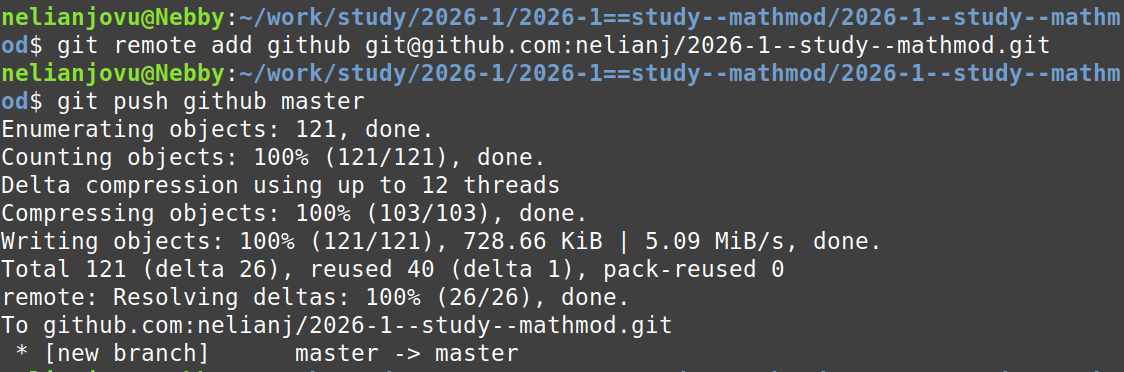
\includegraphics[width=0.7\textwidth,height=\textheight]{image/fig-044.png}

}

\caption{\label{fig-028}создание репозитория}

\end{figure}%
\end{frame}

\begin{frame}{2. Рабочее пространство лабораторной работы}
\phantomsection\label{ux440ux430ux431ux43eux447ux435ux435-ux43fux440ux43eux441ux442ux440ux430ux43dux441ux442ux432ux43e-ux43bux430ux431ux43eux440ux430ux442ux43eux440ux43dux43eux439-ux440ux430ux431ux43eux442ux44b-16}
Я запускаю репозиторий на github(рис. 29)

\begin{figure}

\centering{

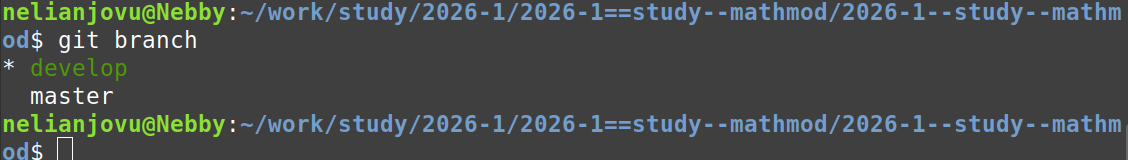
\includegraphics[width=0.7\textwidth,height=\textheight]{image/fig-045.png}

}

\caption{\label{fig-029}запуск репозитория}

\end{figure}%
\end{frame}

\begin{frame}{2. Рабочее пространство лабораторной работы}
\phantomsection\label{ux440ux430ux431ux43eux447ux435ux435-ux43fux440ux43eux441ux442ux440ux430ux43dux441ux442ux432ux43e-ux43bux430ux431ux43eux440ux430ux442ux43eux440ux43dux43eux439-ux440ux430ux431ux43eux442ux44b-17}
Я инициализирую git flow и отвечаю на вопрос в соответствии с
инструкциями(рис. 30)

\begin{figure}

\centering{

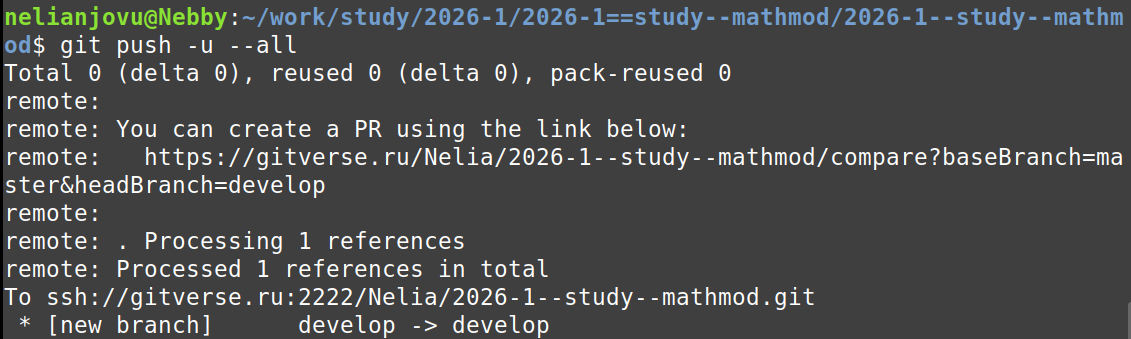
\includegraphics[width=0.7\textwidth,height=\textheight]{image/fig-046.png}

}

\caption{\label{fig-030}инициализация git flow}

\end{figure}%
\end{frame}

\begin{frame}{2. Рабочее пространство лабораторной работы}
\phantomsection\label{ux440ux430ux431ux43eux447ux435ux435-ux43fux440ux43eux441ux442ux440ux430ux43dux441ux442ux432ux43e-ux43bux430ux431ux43eux440ux430ux442ux43eux440ux43dux43eux439-ux440ux430ux431ux43eux442ux44b-18}
Я проверяю и вижу, что нахожусь в ветке разработки. После чего загружаю
весь репозиторий на сервер(рис. 31)

\begin{figure}

\centering{

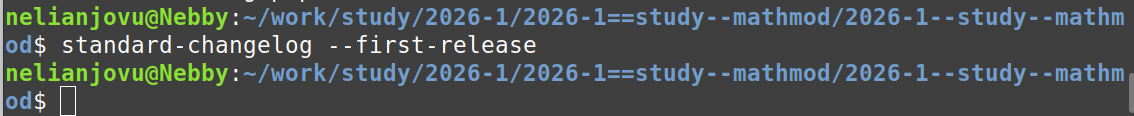
\includegraphics[width=0.7\textwidth,height=\textheight]{image/fig-048.png}

}

\caption{\label{fig-031}загрузка репозитория}

\end{figure}%
\end{frame}

\begin{frame}{2. Рабочее пространство лабораторной работы}
\phantomsection\label{ux440ux430ux431ux43eux447ux435ux435-ux43fux440ux43eux441ux442ux440ux430ux43dux441ux442ux432ux43e-ux43bux430ux431ux43eux440ux430ux442ux43eux440ux43dux43eux439-ux440ux430ux431ux43eux442ux44b-19}
Я создаю релиз с версией 1.0.0 и создаю журнал изменений(рис. 32)

\begin{figure}

\centering{

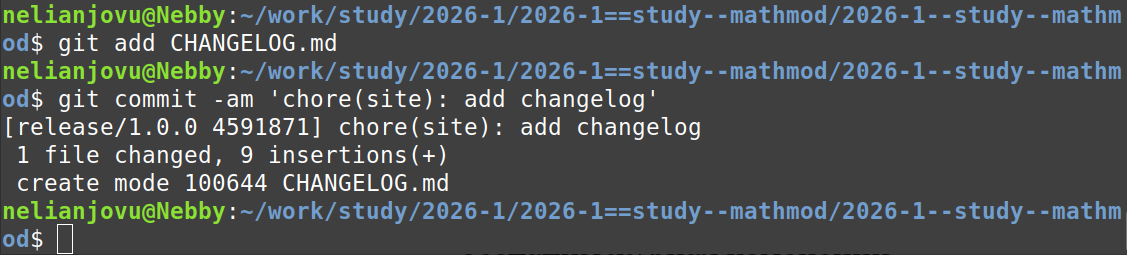
\includegraphics[width=0.7\textwidth,height=\textheight]{image/fig-049.png}

}

\caption{\label{fig-032}создание релиз}

\end{figure}%
\end{frame}

\begin{frame}{2. Рабочее пространство лабораторной работы}
\phantomsection\label{ux440ux430ux431ux43eux447ux435ux435-ux43fux440ux43eux441ux442ux440ux430ux43dux441ux442ux432ux43e-ux43bux430ux431ux43eux440ux430ux442ux43eux440ux43dux43eux439-ux440ux430ux431ux43eux442ux44b-20}
Я добавляю журнал изменений в индекс и загружаю ветку выпуска в основную
ветку(рис. 33)

\begin{figure}

\centering{

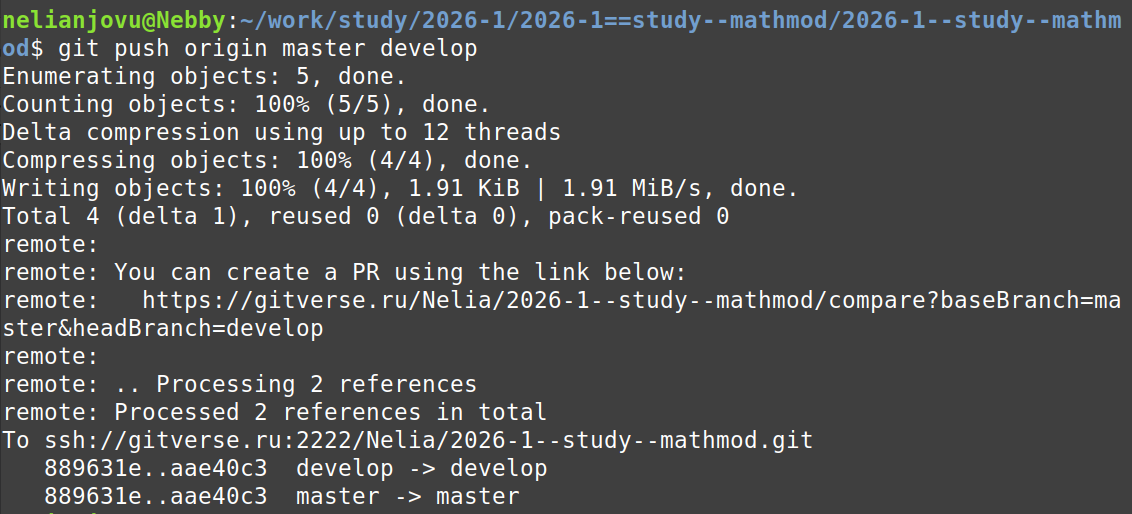
\includegraphics[width=0.7\textwidth,height=\textheight]{image/fig-051.png}

}

\caption{\label{fig-033}загрузка релиз}

\end{figure}%
\end{frame}

\begin{frame}{2. Рабочее пространство лабораторной работы}
\phantomsection\label{ux440ux430ux431ux43eux447ux435ux435-ux43fux440ux43eux441ux442ux440ux430ux43dux441ux442ux432ux43e-ux43bux430ux431ux43eux440ux430ux442ux43eux440ux43dux43eux439-ux440ux430ux431ux43eux442ux44b-21}
После чего я отправляю данные на github(рис. 34)

\begin{figure}

\centering{

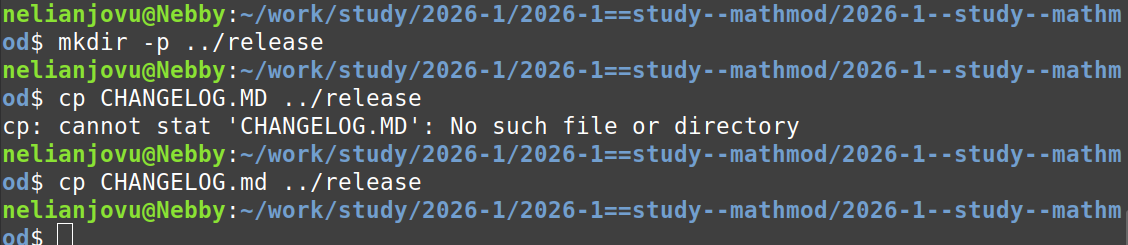
\includegraphics[width=0.7\textwidth,height=\textheight]{image/fig-053.png}

}

\caption{\label{fig-034}отправка данных}

\end{figure}%
\end{frame}

\begin{frame}{2. Рабочее пространство лабораторной работы}
\phantomsection\label{ux440ux430ux431ux43eux447ux435ux435-ux43fux440ux43eux441ux442ux440ux430ux43dux441ux442ux432ux43e-ux43bux430ux431ux43eux440ux430ux442ux43eux440ux43dux43eux439-ux440ux430ux431ux43eux442ux44b-22}
Я копирую CHANGELOG.md в каталог релизов(рис. 35)

\begin{figure}

\centering{

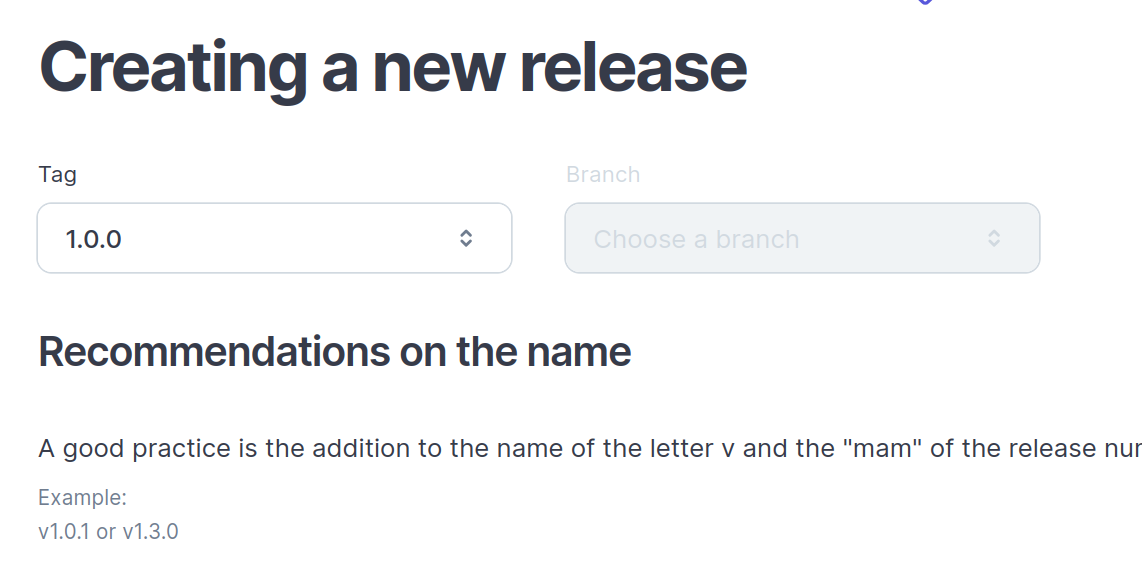
\includegraphics[width=0.7\textwidth,height=\textheight]{image/fig-054.png}

}

\caption{\label{fig-035}копирование файла}

\end{figure}%
\end{frame}

\begin{frame}{2. Рабочее пространство лабораторной работы}
\phantomsection\label{ux440ux430ux431ux43eux447ux435ux435-ux43fux440ux43eux441ux442ux440ux430ux43dux441ux442ux432ux43e-ux43bux430ux431ux43eux440ux430ux442ux43eux440ux43dux43eux439-ux440ux430ux431ux43eux442ux44b-23}
Я создаю релиз вручную на gitverse(рис. 36)

\begin{figure}

\centering{

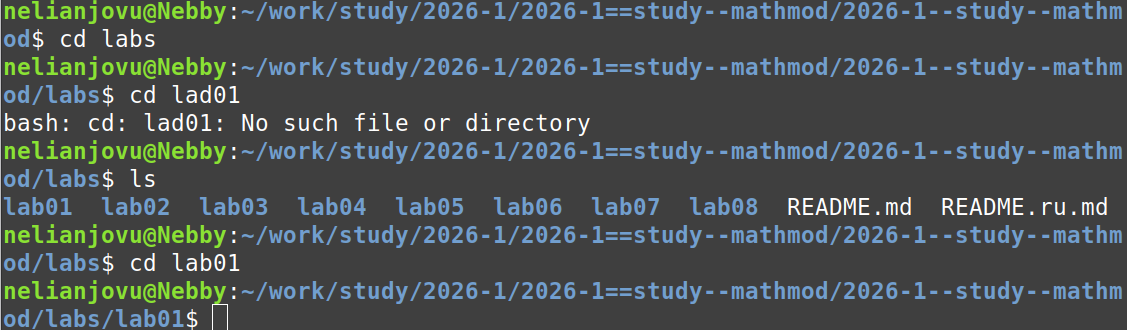
\includegraphics[width=0.7\textwidth,height=\textheight]{image/fig-055.png}

}

\caption{\label{fig-036}создание релиз}

\end{figure}%
\end{frame}

\begin{frame}{3. Создание проекта DrWatson для лабораторных}
\phantomsection\label{ux441ux43eux437ux434ux430ux43dux438ux435-ux43fux440ux43eux435ux43aux442ux430-drwatson-ux434ux43bux44f-ux43bux430ux431ux43eux440ux430ux442ux43eux440ux43dux44bux445}
Я захожу в каталог lab01, устанавливаю julia и запускаю его(рис. 37)

\begin{figure}

\centering{

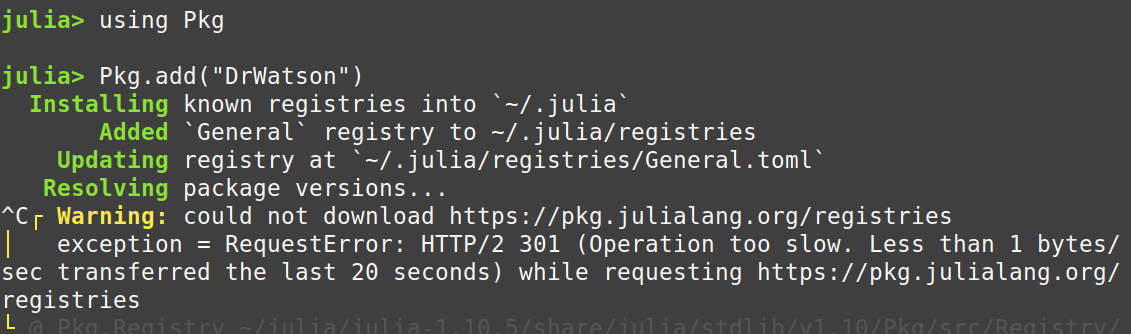
\includegraphics[width=0.7\textwidth,height=\textheight]{image/fig-057.png}

}

\caption{\label{fig-037}запуск julia}

\end{figure}%
\end{frame}

\begin{frame}{3. Создание проекта DrWatson для лабораторных}
\phantomsection\label{ux441ux43eux437ux434ux430ux43dux438ux435-ux43fux440ux43eux435ux43aux442ux430-drwatson-ux434ux43bux44f-ux43bux430ux431ux43eux440ux430ux442ux43eux440ux43dux44bux445-1}
Я создаю структуру проекта, используя пакет DrWatson в Julia's REPL(рис.
38)

\begin{figure}

\centering{

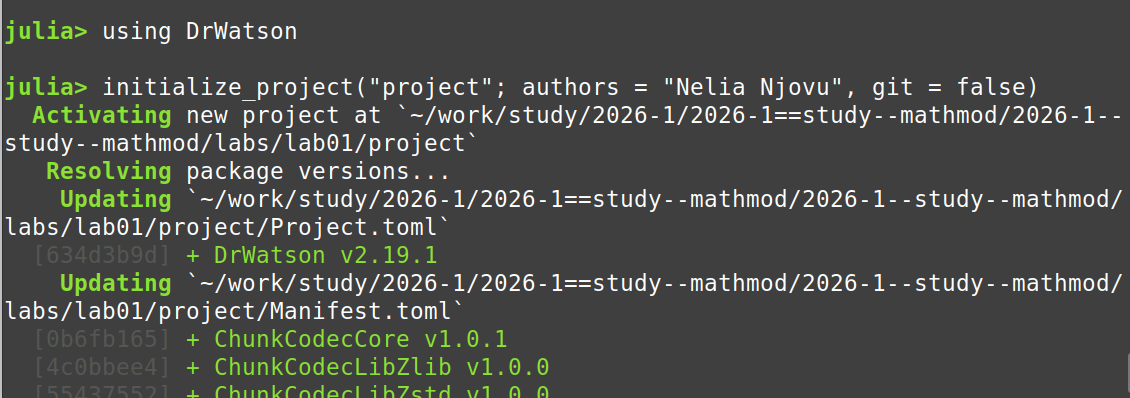
\includegraphics[width=0.7\textwidth,height=\textheight]{image/fig-058.png}

}

\caption{\label{fig-038}создание структуру}

\end{figure}%
\end{frame}

\begin{frame}{3. Создание проекта DrWatson для лабораторных}
\phantomsection\label{ux441ux43eux437ux434ux430ux43dux438ux435-ux43fux440ux43eux435ux43aux442ux430-drwatson-ux434ux43bux44f-ux43bux430ux431ux43eux440ux430ux442ux43eux440ux43dux44bux445-2}
Я создаю jl-файл, копирую и вставляю скрипт из руководства пользователя.
Скрипт настраивает всю структуру папок. После этого я запускаю файл(рис.
39)

\begin{figure}

\centering{

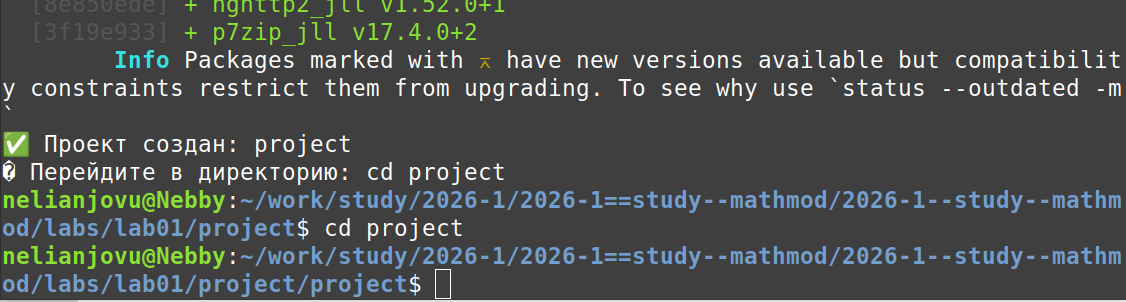
\includegraphics[width=0.7\textwidth,height=\textheight]{image/fig-060.png}

}

\caption{\label{fig-039a}создание первого jl-файла}

\end{figure}%
\end{frame}

\begin{frame}{3. Создание проекта DrWatson для лабораторных}
\phantomsection\label{ux441ux43eux437ux434ux430ux43dux438ux435-ux43fux440ux43eux435ux43aux442ux430-drwatson-ux434ux43bux44f-ux43bux430ux431ux43eux440ux430ux442ux43eux440ux43dux44bux445-3}
\begin{figure}

\centering{

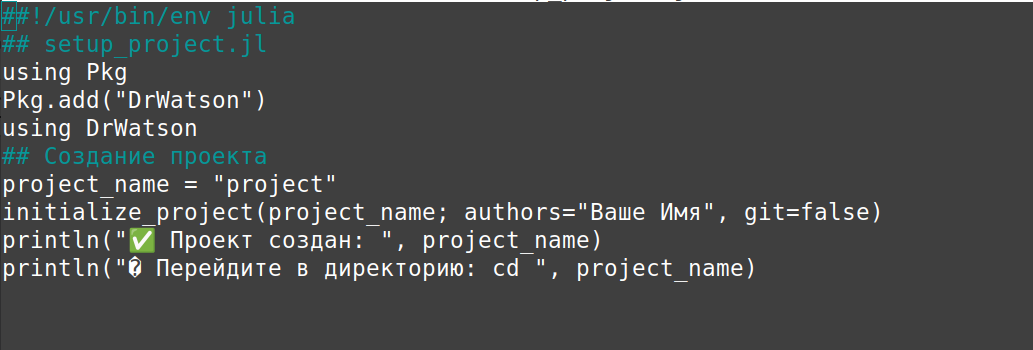
\includegraphics[width=0.7\textwidth,height=\textheight]{image/fig-061.png}

}

\caption{\label{fig-039b}создание первого jl-файла}

\end{figure}%
\end{frame}

\begin{frame}{3. Создание проекта DrWatson для лабораторных}
\phantomsection\label{ux441ux43eux437ux434ux430ux43dux438ux435-ux43fux440ux43eux435ux43aux442ux430-drwatson-ux434ux43bux44f-ux43bux430ux431ux43eux440ux430ux442ux43eux440ux43dux44bux445-4}
Я создаю jl-файл с именем add\_packages, копирую и вставляю скрипт из
руководства. Скрипт Этот скрипт устанавливает все пакеты Julia. После
этого я запускаю файл(рис. 40)

\begin{figure}

\centering{

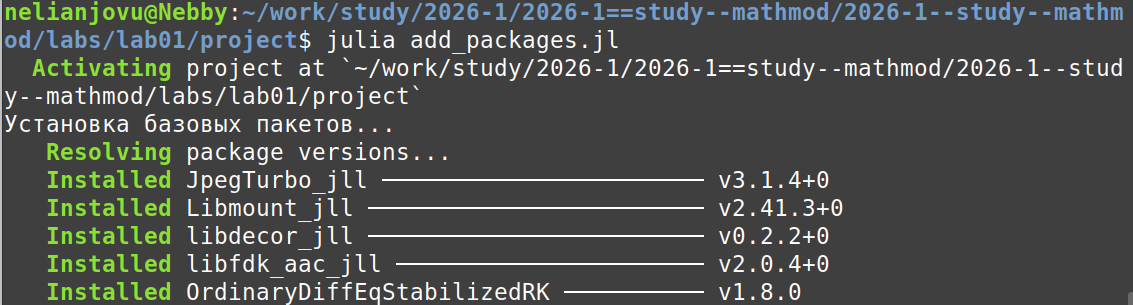
\includegraphics[width=0.7\textwidth,height=\textheight]{image/fig-063.png}

}

\caption{\label{fig-040}создание jl-файла add\_packages}

\end{figure}%
\end{frame}

\begin{frame}{3. Создание проекта DrWatson для лабораторных}
\phantomsection\label{ux441ux43eux437ux434ux430ux43dux438ux435-ux43fux440ux43eux435ux43aux442ux430-drwatson-ux434ux43bux44f-ux43bux430ux431ux43eux440ux430ux442ux43eux440ux43dux44bux445-5}
После установки я проверяю свою окончательную структуру проекта, и она
выглядит точно так же, как в руководстве(рис. 41)

\begin{figure}

\centering{

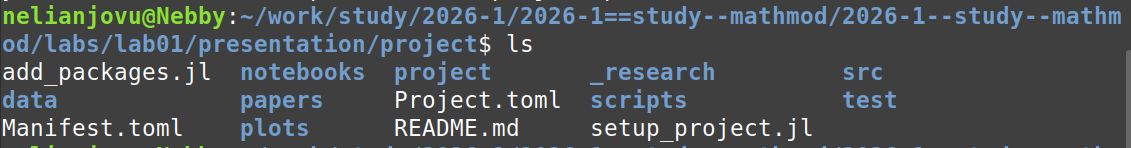
\includegraphics[width=0.7\textwidth,height=\textheight]{image/fig-066.png}

}

\caption{\label{fig-041}проверка структуру}

\end{figure}%
\end{frame}

\begin{frame}{3. Создание проекта DrWatson для лабораторных}
\phantomsection\label{ux441ux43eux437ux434ux430ux43dux438ux435-ux43fux440ux43eux435ux43aux442ux430-drwatson-ux434ux43bux44f-ux43bux430ux431ux43eux440ux430ux442ux43eux440ux43dux44bux445-6}
Я создаю jl-файл с именем 01\_exponential\_growth, копирую и вставляю
скрипт из руководства. Этот скрипт решает и визуализирует модель
экспоненциального роста(рис. 42)

\begin{figure}

\centering{

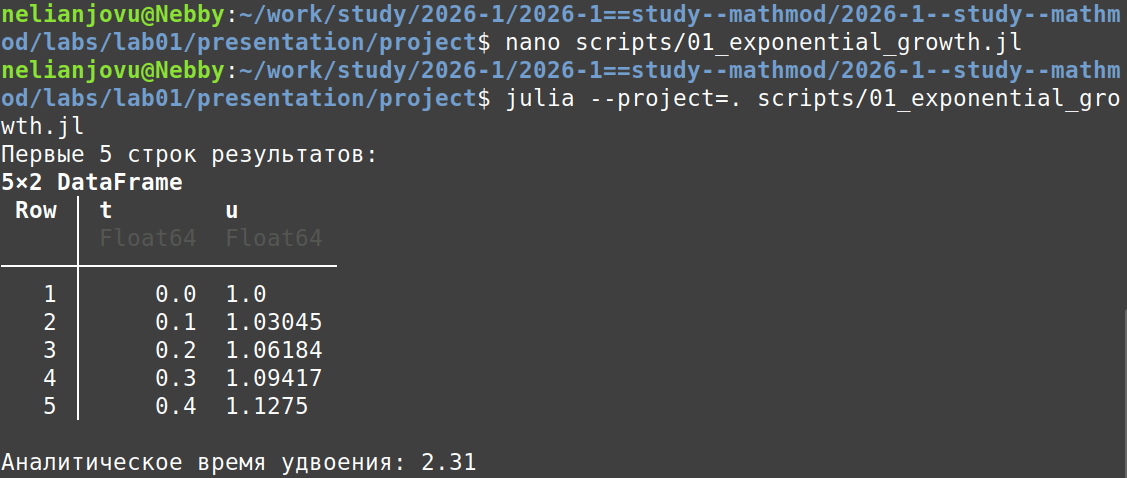
\includegraphics[width=0.7\textwidth,height=\textheight]{image/fig-068.png}

}

\caption{\label{fig-042}создание jl-файла 01\_exponential\_growth}

\end{figure}%
\end{frame}

\begin{frame}{3. Создание проекта DrWatson для лабораторных}
\phantomsection\label{ux441ux43eux437ux434ux430ux43dux438ux435-ux43fux440ux43eux435ux43aux442ux430-drwatson-ux434ux43bux44f-ux43bux430ux431ux43eux440ux430ux442ux43eux440ux43dux44bux445-7}
Полученные графики отображаются в каталоге plots(рис. 43)

\begin{figure}

\centering{

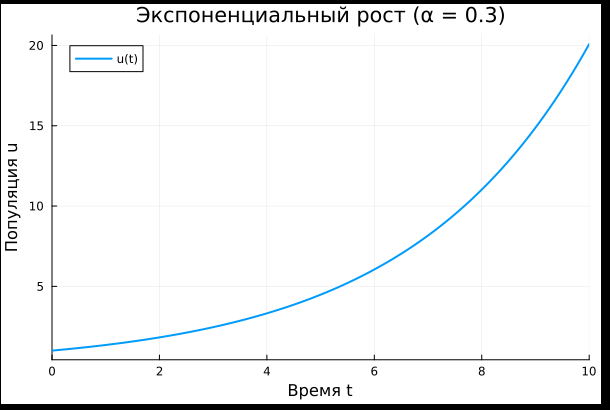
\includegraphics[width=0.7\textwidth,height=\textheight]{image/fig-069.png}

}

\caption{\label{fig-043}графики}

\end{figure}%
\end{frame}

\begin{frame}{4. Модель экспоненциального роста}
\phantomsection\label{ux43cux43eux434ux435ux43bux44c-ux44dux43aux441ux43fux43eux43dux435ux43dux446ux438ux430ux43bux44cux43dux43eux433ux43e-ux440ux43eux441ux442ux430}
Я редактирую скрипт в файле 01\_exponential\_growth. Новый скрипт
выполняет точно ту же математическую работу, что и предыдущий, за
исключением того, что теперь он написан в грамотном стиле
программирования(рис. 44)

!{[}отредактированный скрипт{]}(image/fig-070\{\#fig-044 width=70\%\}
\end{frame}

\begin{frame}{4. Модель экспоненциального роста}
\phantomsection\label{ux43cux43eux434ux435ux43bux44c-ux44dux43aux441ux43fux43eux43dux435ux43dux446ux438ux430ux43bux44cux43dux43eux433ux43e-ux440ux43eux441ux442ux430-1}
Я создаю jl-файл с именем tangle, копирую и вставляю скрипт из
руководства. Этот скрипт представляет собой конвертер, который
использует файлы Julia literate (с комментариями и кодом) и
автоматически генерирует три разных формата: .jl; .qmd; .ipynb(рис. 45)

\begin{figure}

\centering{

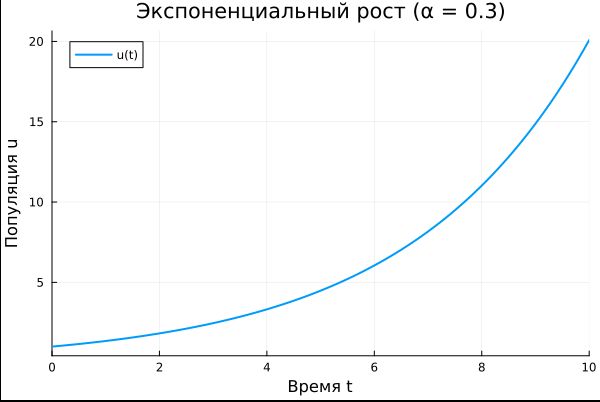
\includegraphics[width=0.7\textwidth,height=\textheight]{image/fig-072.png}

}

\caption{\label{fig-045}создание jl-файла tangle}

\end{figure}%
\end{frame}

\begin{frame}{4. Модель экспоненциального роста}
\phantomsection\label{ux43cux43eux434ux435ux43bux44c-ux44dux43aux441ux43fux43eux43dux435ux43dux446ux438ux430ux43bux44cux43dux43eux433ux43e-ux440ux43eux441ux442ux430-2}
Я проверяю, был ли создан файл ipynb(рис. 46)

\begin{figure}

\centering{

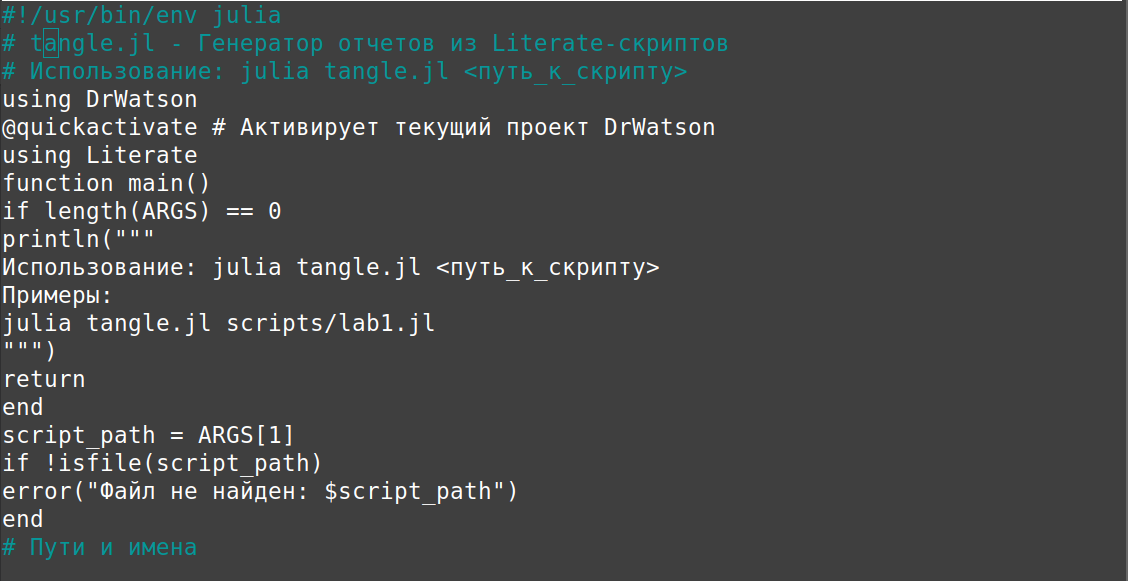
\includegraphics[width=0.7\textwidth,height=\textheight]{image/fig-073.png}

}

\caption{\label{fig-046}проверка файл}

\end{figure}%
\end{frame}

\begin{frame}{4. Модель экспоненциального роста}
\phantomsection\label{ux43cux43eux434ux435ux43bux44c-ux44dux43aux441ux43fux43eux43dux435ux43dux446ux438ux430ux43bux44cux43dux43eux433ux43e-ux440ux43eux441ux442ux430-3}
В каталоге отчетов, в файле \_quarto.yml, я включаю поддержку кода
julia(рис. 47)

\begin{figure}

\centering{

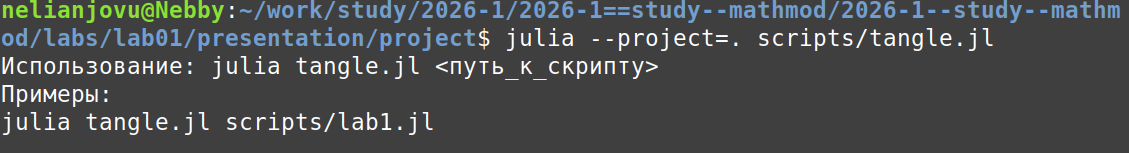
\includegraphics[width=0.7\textwidth,height=\textheight]{image/fig-075.png}

}

\caption{\label{fig-047}редактирование файла \_quarto.yml}

\end{figure}%
\end{frame}

\begin{frame}{4. Модель экспоненциального роста}
\phantomsection\label{ux43cux43eux434ux435ux43bux44c-ux44dux43aux441ux43fux43eux43dux435ux43dux446ux438ux430ux43bux44cux43dux43eux433ux43e-ux440ux43eux441ux442ux430-4}
В преамбуле к preview.tex я подключаю пакет juliamono(рис. 48)

\begin{figure}

\centering{

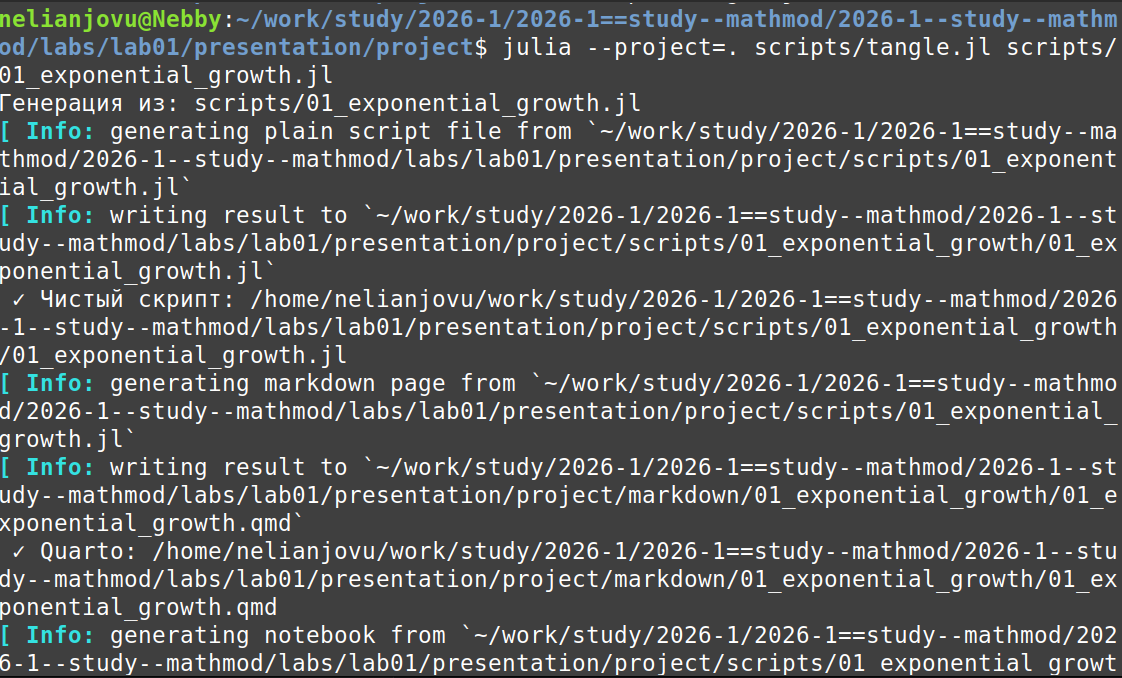
\includegraphics[width=0.7\textwidth,height=\textheight]{image/fig-076.png}

}

\caption{\label{fig-048}пакет juliamono}

\end{figure}%
\end{frame}

\begin{frame}{4. Модель экспоненциального роста}
\phantomsection\label{ux43cux43eux434ux435ux43bux44c-ux44dux43aux441ux43fux43eux43dux435ux43dux446ux438ux430ux43bux44cux43dux43eux433ux43e-ux440ux43eux441ux442ux430-5}
Я создаю jl-файл с именем 02\_exponential\_growth, копирую и вставляю
скрипт из руководства. Этот скрипт основан на предыдущей версии, но
добавляет систематическую проверку параметров и сравнительный анализ
производительности(рис. 49)

\begin{figure}

\centering{

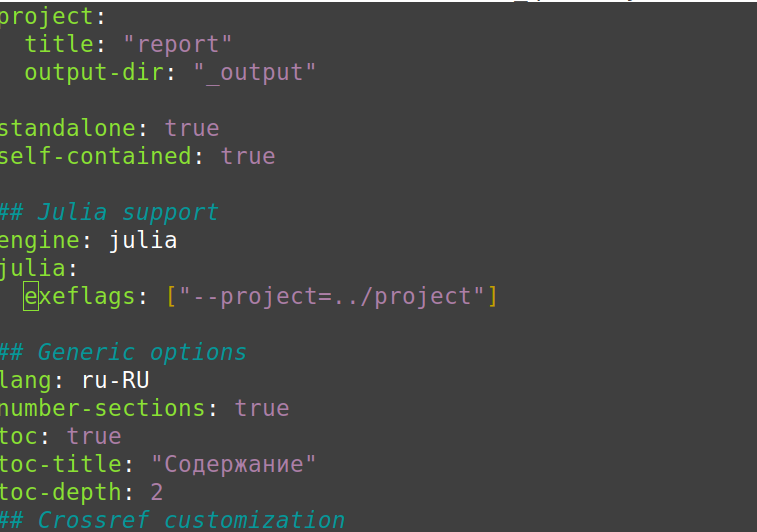
\includegraphics[width=0.7\textwidth,height=\textheight]{image/fig-079.png}

}

\caption{\label{fig-049}создание jl-файла 02\_exponential\_growth}

\end{figure}%
\end{frame}

\begin{frame}{4. Модель экспоненциального роста}
\phantomsection\label{ux43cux43eux434ux435ux43bux44c-ux44dux43aux441ux43fux43eux43dux435ux43dux446ux438ux430ux43bux44cux43dux43eux433ux43e-ux440ux43eux441ux442ux430-6}
Используя tangle, я создаю три новых файла и открываю файл ipynb, чтобы
проверить его(рис. 50)

\begin{figure}

\centering{

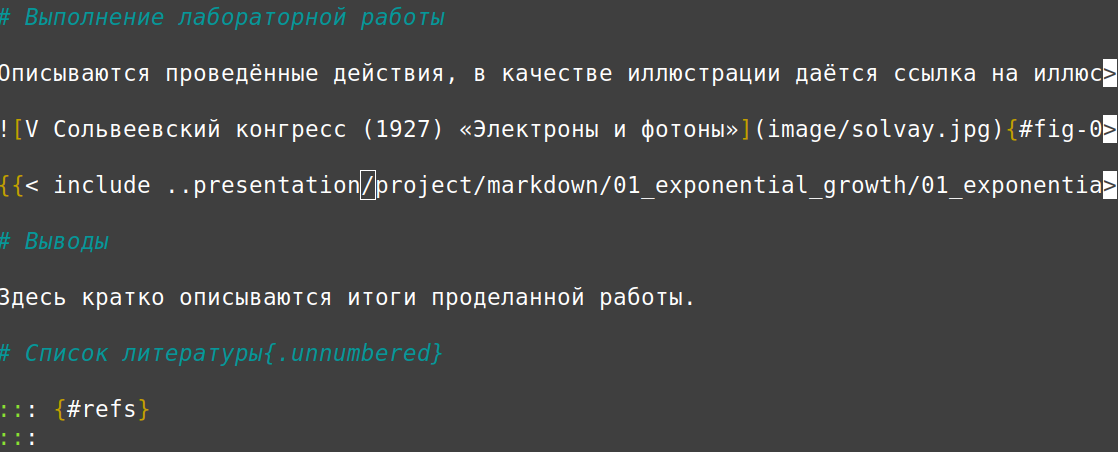
\includegraphics[width=0.7\textwidth,height=\textheight]{image/fig-081.png}

}

\caption{\label{fig-050}создание новых файлов}

\end{figure}%
\end{frame}

\begin{frame}{Выводы}
\phantomsection\label{ux432ux44bux432ux43eux434ux44b}
Делая эту лабораторную работу, я изучила модель экспоненциального роста
и проверила параметрическое исследование влияния коэффициента роста α на
динамику системы, а также освоила современные практики воспроизводимых
исследований (литературное программирование, DrWatson, Git).
\end{frame}

\begin{frame}{Список литературы}
\phantomsection\label{ux441ux43fux438ux441ux43eux43a-ux43bux438ux442ux435ux440ux430ux442ux443ux440ux44b}
\begin{enumerate}[<+->]
\item
  A Multi-Language Computing Environment for Literate Programming and
  Reproducible Research / E. Schulte {[}et al.{]} // Journal of
  Statistical Software. --- 2012. --- Vol. 46, no. 3. --- ISSN
  1548-7660. --- DOI: 10.18637/jss.v046.i03.
\item
  Knuth D. E. Literate Programming // The Computer Journal. --- 1984.
  --- Feb.~--- Vol. 27, no. 2. --- P. 97--111. --- ISSN 1460-2067. ---
  DOI: 10.1093/comjnl/27.2.97.
\item
  The Story in the Notebook / M. B. Kery {[}et al.{]} // Proceedings of
  the 2018 CHI Conference on Human Factors in Computing Systems. ---
  ACM, 04/2018. --- P. 1--11. --- DOI: 10.1145/3173574.3173748.
\end{enumerate}
\end{frame}



\end{document}
